\documentclass[parskip=full]{report} % enables german formatting

\usepackage[utf8]{inputenc} % use utf8 file encoding for TeX sources
\usepackage[T1]{fontenc} % avoid garbled Unicode text in pdf
\usepackage[english]{babel} % english hyphenation, quotes, etc
\usepackage{hyperref} % detailed hyperlink/pdf configuration
\usepackage{setspace} % to set spacings between lines
\usepackage{parskip}
\usepackage{graphicx}
\usepackage{rotating}
\usepackage{amsmath}
\usepackage{pifont,mdframed}

% used for warning boxes in the text
\newenvironment{warning}
  {\par\begin{mdframed}[linewidth=1pt,linecolor=red]%
    \begin{list}{}{\leftmargin=1cm
                   \labelwidth=\leftmargin}\item[\Large\ding{43}]}
  {\end{list}\end{mdframed}\par}


%Simon: Hinzufügen des Titelbildes
\usepackage{titlepic}


\hypersetup{ % ‘texdoc hyperref‘ for options
pdftitle={PSE},
bookmarks=true,
}
\usepackage{csquotes} % provides \enquote{} macro for "quotes"

\usepackage[section]{placeins} % Bilder sollen nicht in andere Kapitel ragen

% Abbildungen mit Kapiteln numerieren
\usepackage{chngcntr}
\counterwithin{figure}{section}

% Rahmen um Abbildugen
\usepackage{xcolor}
\usepackage[export]{adjustbox}


\title{Konfigurator für OSM-Datenaufbereitungs-Prozesse für die Verkehrsnachfragemodellierung \\}



\author{
\vspace{5mm}\\
Felix Weik\\ Jan-Philipp Hansen\\ Karl Bernhard\\ Pascal Dawideit\\ Simon Schupp}
\date{December 2022}

% open street map picture in the titlepage
\titlepic{
\begin{figure}[!htb]
    \centering
    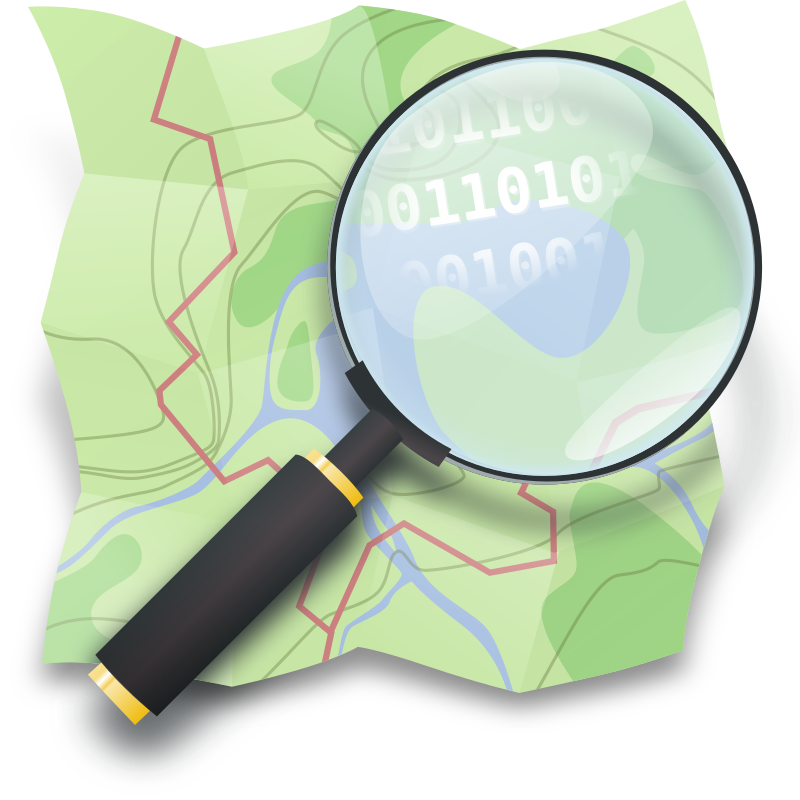
\includegraphics[width=7cm]{pictures/Openstreetmap_logo.png}
    \caption{Uhrheber: Ken Vermette, Lizenz: \protect\href{https://creativecommons.org/licenses/by-sa/3.0/}{CC BY-SA 3.0}}
\end{figure}
}

\begin{document}

\maketitle

\tableofcontents


\chapter{Introduction}

\section{Introduction to the product}
Whether it’s biking to college or driving to the supermarket, traffic
affects us all. all. This product generates from geodata of the free
project ‘OpenStreetMap’ (OSM) a numerical ranking of the
attractiveness of geographic locations. A main focus is the
configurability of the generation of this score. Traffic planners can
easily generate the right data for their traffic forecasting models.

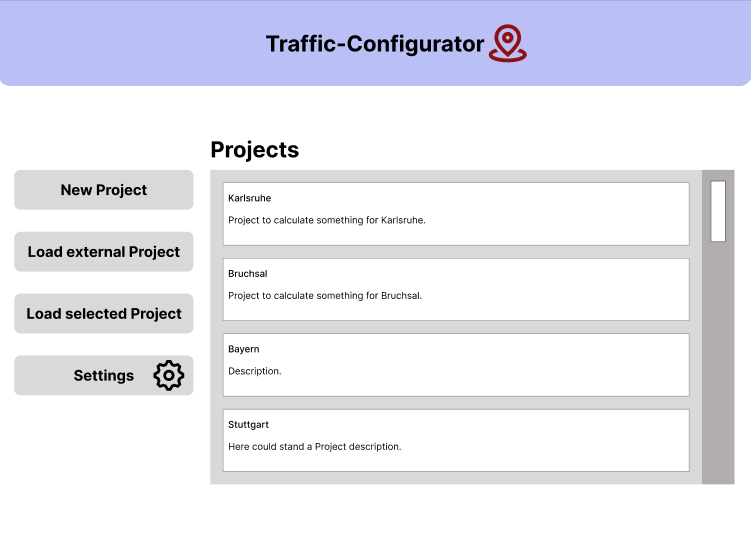
\includegraphics[width=0.450\linewidth]{{pictures/Project_Screen}.png} 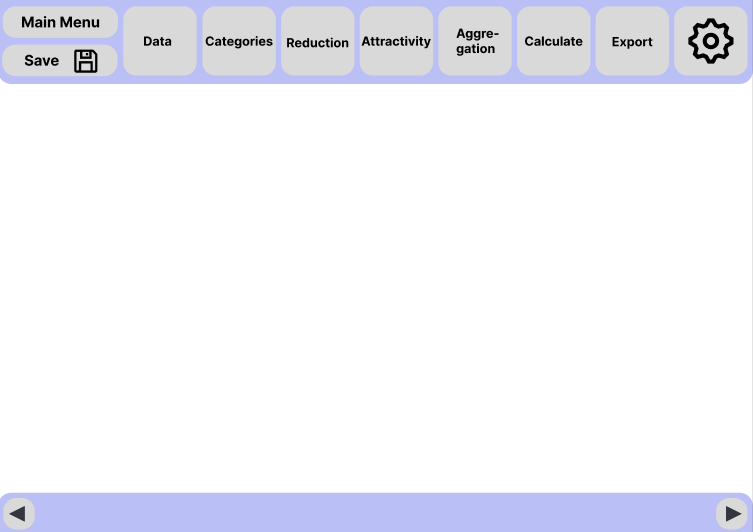
\includegraphics[width=0.450\linewidth]{{pictures/Inside_Project_Screen}.png}

This project is getting developed in the context of the lecture “Praxis der
Softwareentwicklung(PSE)” at the University KIT in 2022,the waterfall
model with feedback was used to develop the project.
For each of this phase you can find the documentation in the
corresponding subfolder, in the 
\href{https://github.com/LuposX/KonfiguratorFuerOSMDaten}{github} , most of the documentation is in german.

\section{Introduction to the design booklet}
The purpose of this document is to communicate our design for the product described above. It describes and justifies the design decisions made in the design phase. The design booklet lays the foundation for the implementation phase.\\
Firstly in the chapter 'Requirement Changes' we lay down how our requirements changed since the submission of our specifications sheet. In 'Package Structure' the structure of the packages and classes is presented using class-diagrams. The chapter 'Software Patterns' explains the software patterns used in the class diagrams mentioned above. The chapter 'Sequence Diagram' uses a sequence diagram as an example to show how the model, view and control packages work together. The details of the design presented in 'Package Structure' are shown in the chapter 'Class Descriptions'. It contains a description of all classes and public methods. The chapter 'Libraries' lists the libraries used in our drafts and justifies there usage.


\chapter{Requirement Changes}
The specification sheet defined the requirements of our product. Because of changes in our knowledge about the feasibility of some of the requirements, we made some changes to them. In this chapter we will list and explain those changes.

\section*{Cut-Out Map}
A map is added to the application. The map visualizes the cut-out data given by the user. The user can press a button and the map is displayed afterwards. The user can also export this map to the computer. Those features can be defined as follows:
\begin{itemize}
    \item <WK9> The user can open a map to visualize the cut-out files
    \item <WK10> The user can export the cut-out map
\end{itemize}
Those feature have the priority ''desired criterion''. We decided to ass those features, because add a lot to the user experience, while not adding much changes in the design.

\section*{Download Repository}
The user can decide to download OSM-data from a repository. In the specifications we decided, the user defines which OSM-data he wants to download by entering a URL. This is technically unpractical. Therefore we decided to automatically download the OSM-data, that is surrounded by the already given cut-out files. This change does only affect the alternative 2a in the use case A6 in the specifications.

\section*{Delete Project}
In the specifications there is never mentioned, that the user can delete projects. Because this is a fundamental feature of our product, we decided to add it. This change of requirements is a extension of the criterion MK1 in the specifications.

\section*{Calculation of Attractivity with Tags}
WK7 of the specifications states as a desired criterion that attractivity attributes may be calculated in dependency to OSM-tags. The problem is, that tags come in more variants than we thought. For instance it is hard to give a value to the tag ''wheelchair=limited''. Hence we decided to remove this feature and not cover it in our designs.

\section*{Arbitrary Tag-Filters}
WK2 of the specifications states, that the user might use arbitrary logical statements to define the tag filters of the categories. This criterion was not supposed to be in the specifications, but was left there accidentally.



\chapter{Package Structure}
In this chapter we will go over and explain the structure of the product. Firstly the package structure is explained. This is done using package and class diagrams. Those diagrams do also contain the complete structure of all the classes used in our design. The class diagrams form the foundation for all the upcoming chapters. In chapter \ref{sec::descriptions} the classes and methods of the class diagrams will be described in more detail.

\section{Model-View-Controller} \label{sec::mvc}
This project is organized in three underlying units: Model, view and control. This structure is based on the architectural "Model-View-Controller" pattern (short MVC). 
The model is responsible for the organisation of the data of the application. The view manages the user interface (UI). The task of the control-unit is to allow a consistent communication between the two above mentioned units. The communication is always initialized by the view. It sends requests to the control and the control forwards them to the model after checking.\\
We decided to use this variant of the MVC, because it makes our project easily changeable. For instance, building in a totally new view could be easily done.\\
In figure \ref{fig:mvc} you can see the structure of the packages. It shows the associations between them.


\section{Package View}
The \hyperlink{view}{view} is then further divided into four subpackages: \hyperlink{popups}{popups}, \hyperlink{states}{states}, \hyperlink{toplevelframes}{toplevelframes} and \hyperlink{utilityframes}{utilityframes}. The last three all have access to pupup. In addition, states has access to the toplevelframes package and toplevelframes itself has access to utilityframes. Overall, the view is responsible for displaying data for the user and let him edit those. Popup displays pop-ups that occur during usage. States is responsible for which phases should be displayed and when it should be displayed. Toplevelframes includes the phases to be displayed themselves and utilityframes is responsible for displaying sub-frames. For more information about the packages, read the documentation of the classes within the packages.

\section{Package Controller}
The \hyperlink{controller}{controller} is not further subdivided and takes care of the communication between view and model and initializes the other packages.

\section{Package Model}
The \hyperlink{model}{model} is divided into \hyperlink{application}{application}, \hyperlink{project}{project} and \hyperlink{parser}{parser}, with project being further subdivided into \hyperlink{configuration}{configuration} and \hyperlink{calculation}{calculation}. The application has access to the project and the project has access to the parser. In addition, calculation has access to the configuration. The model is overall responsible for storing the data. The application package is responsible for project-independent data and the parser for importing data. The configuration saves the data that arises during the individual phases and the calculation in turn saves those that occur during the calculation. For more information about the packages, read the documentation of the classes within the packages.

\section{Diagrams}

\hypertarget{mvc}{
\begin{figure}[hbt!]
  \centering
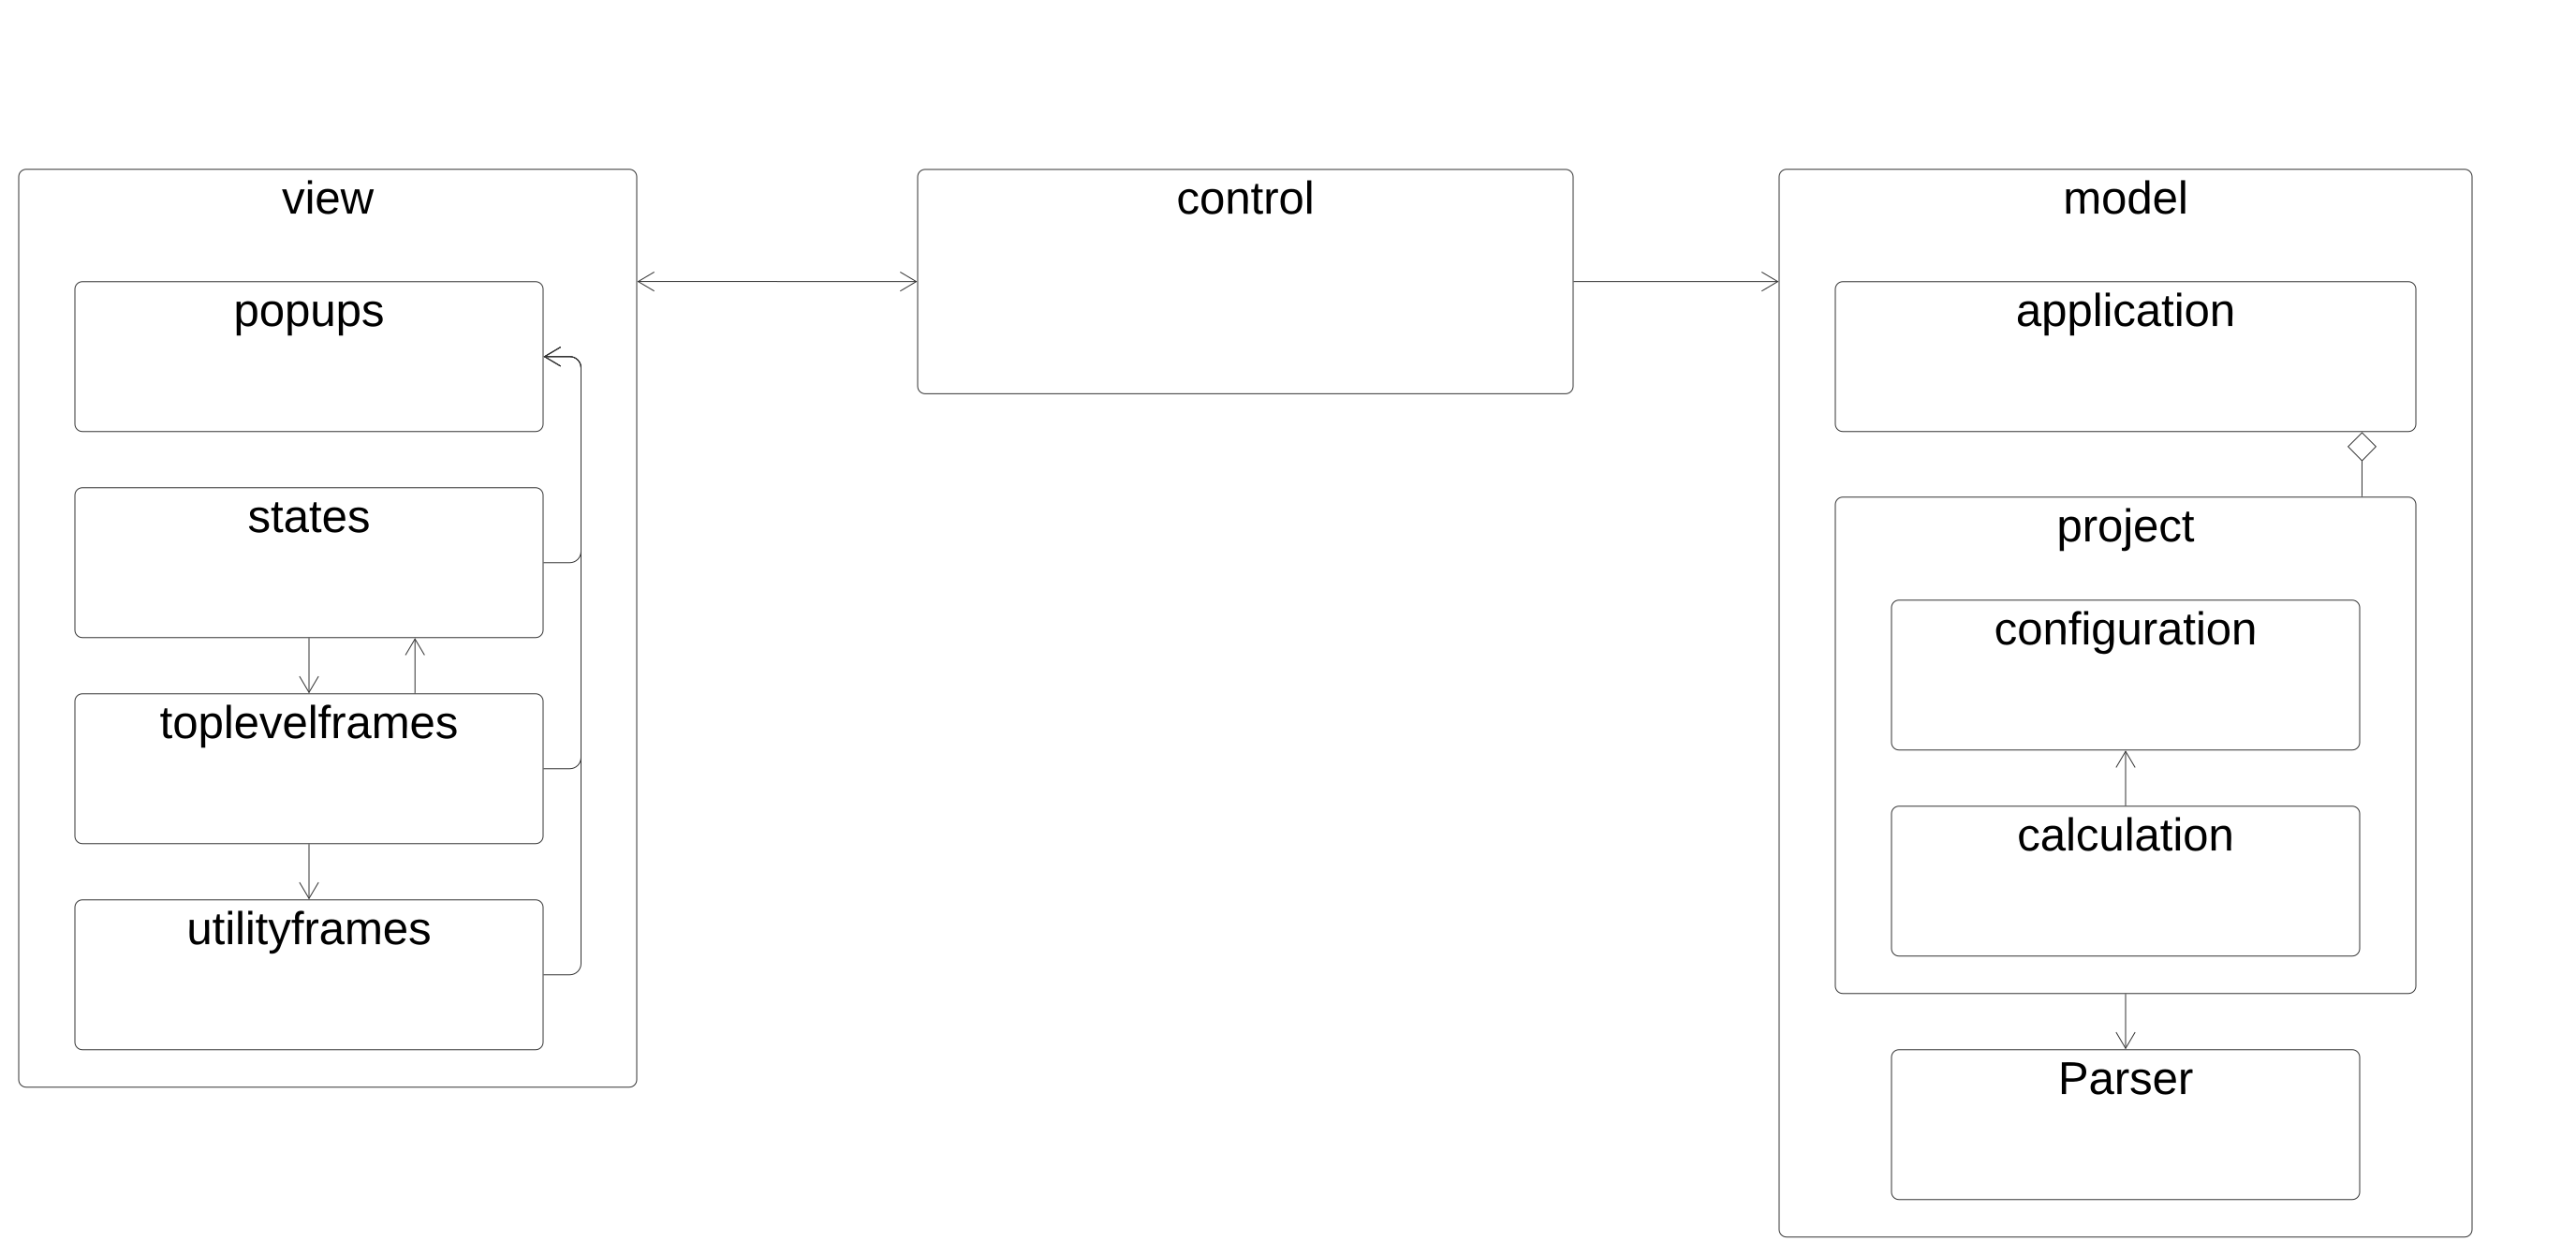
\includegraphics[width=0.8\textwidth]
        {pictures/mvc.png}
  \caption{Model-View-Control Packages}
  \label{fig:mvc}
\end{figure}
}

\hypertarget{controller}{
\begin{figure}[hbt!]
  \centering
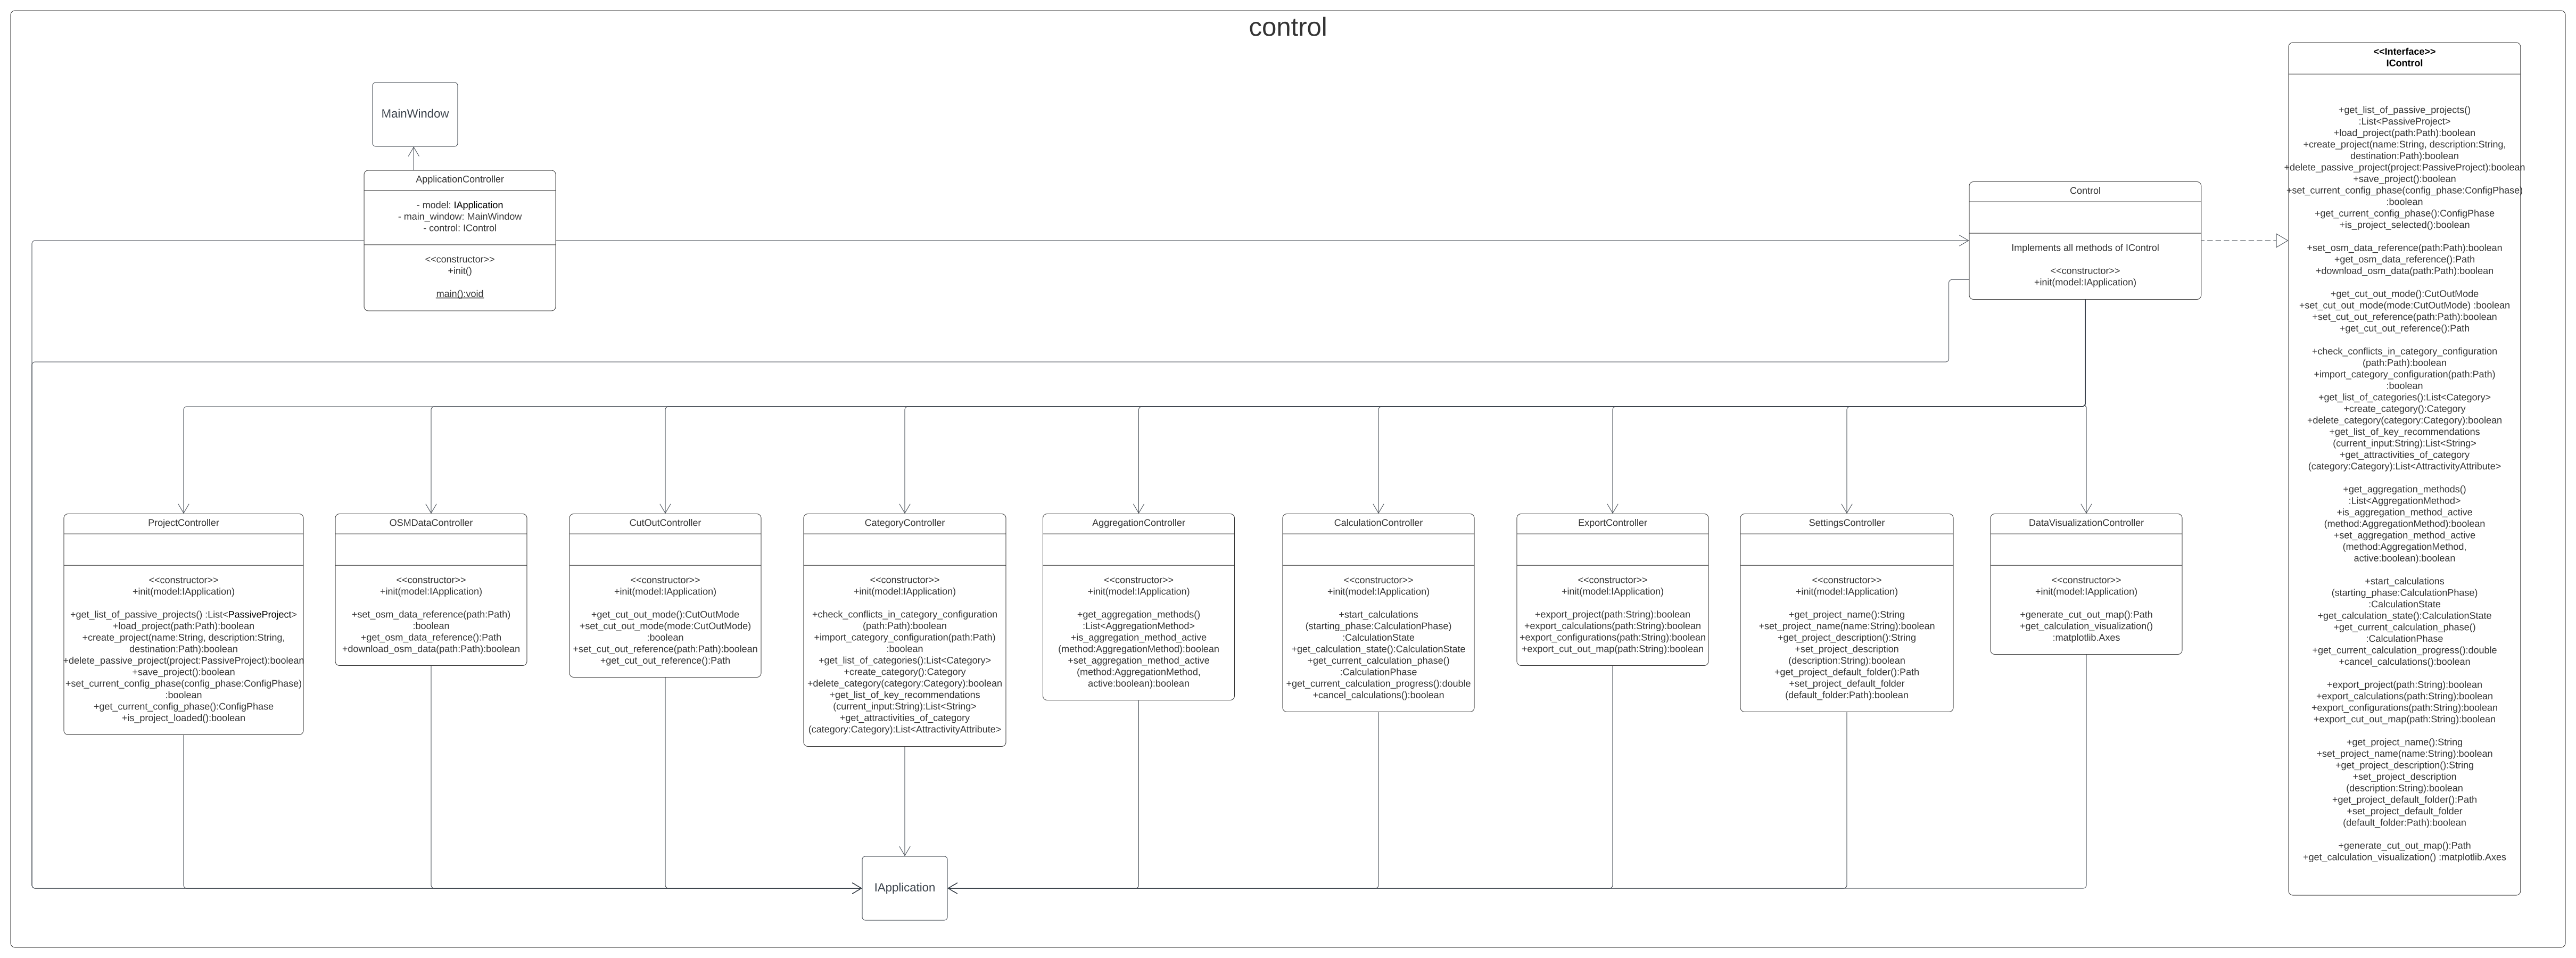
\includegraphics[width=0.8\textwidth]
        {pictures/controller.png}
  \caption{Package: controller}
  \label{fig:mvc}
\end{figure}
}

\hypertarget{view}{
\begin{figure}[hbt!]
  \centering
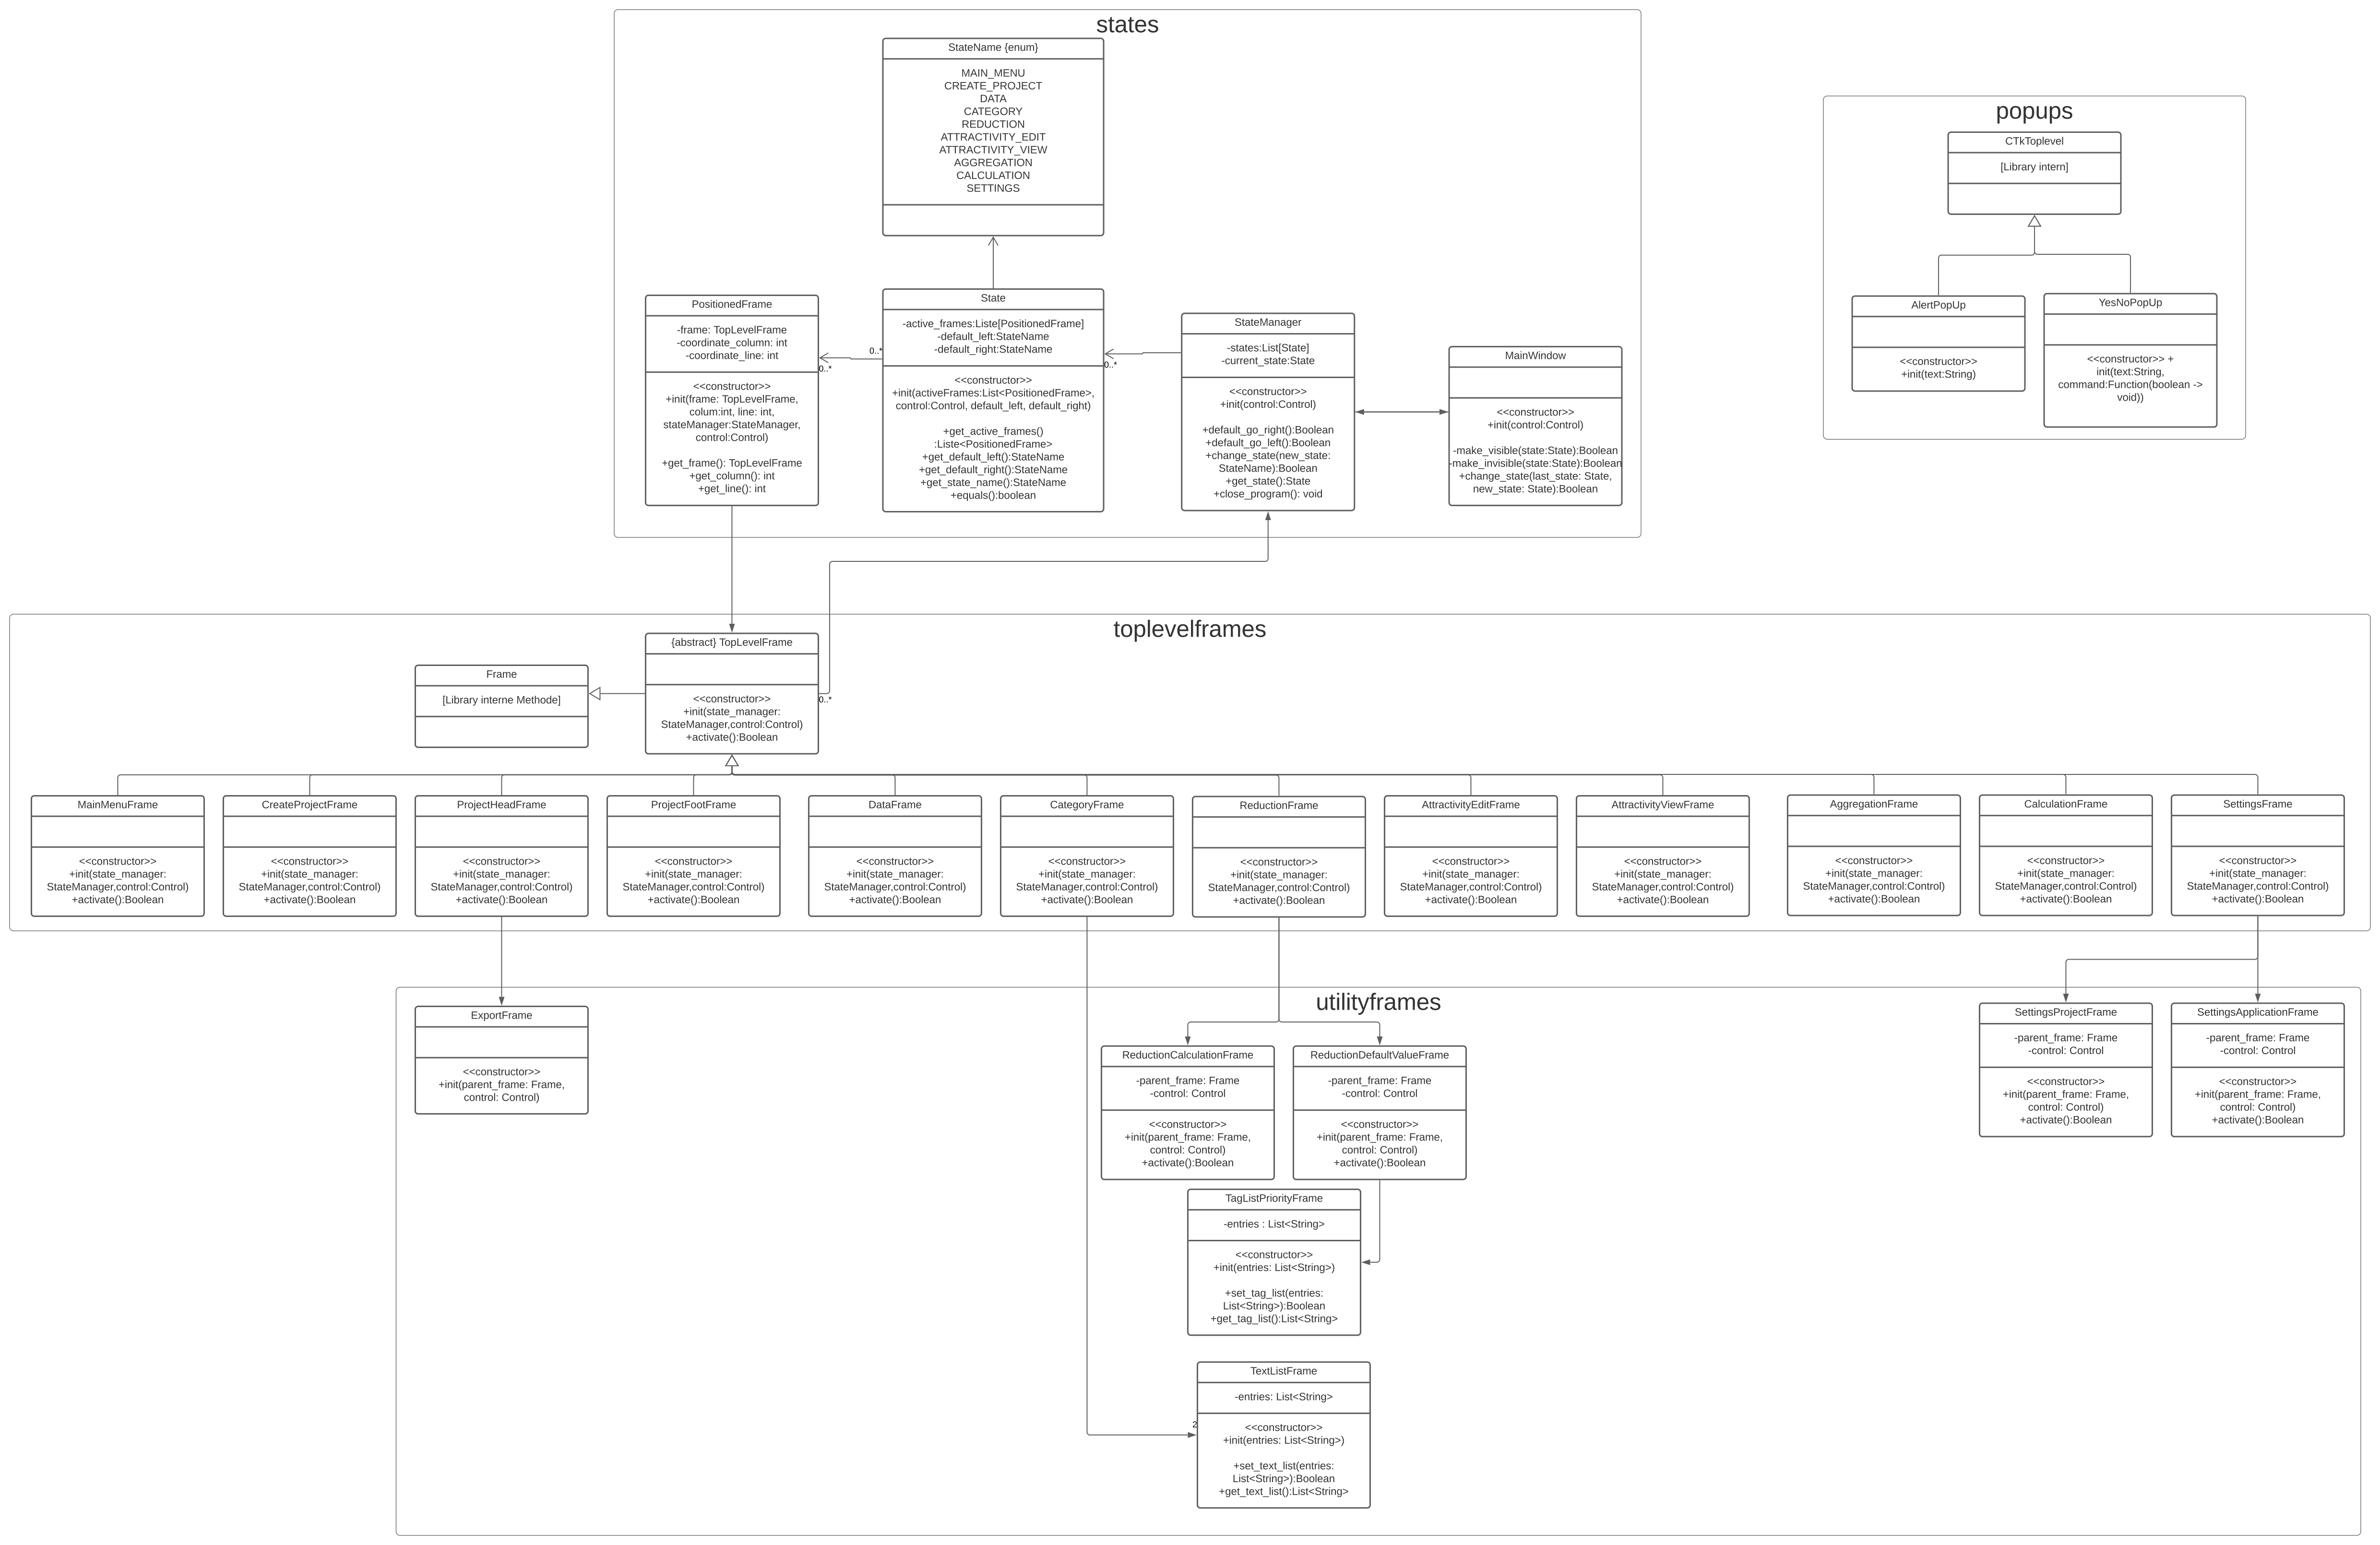
\includegraphics[width=0.8\textwidth]
        {pictures/view.png}
  \caption{Package: view}
  \label{fig:mvc}
\end{figure}
}

\hypertarget{model}{
\begin{figure}[hbt!]
  \centering
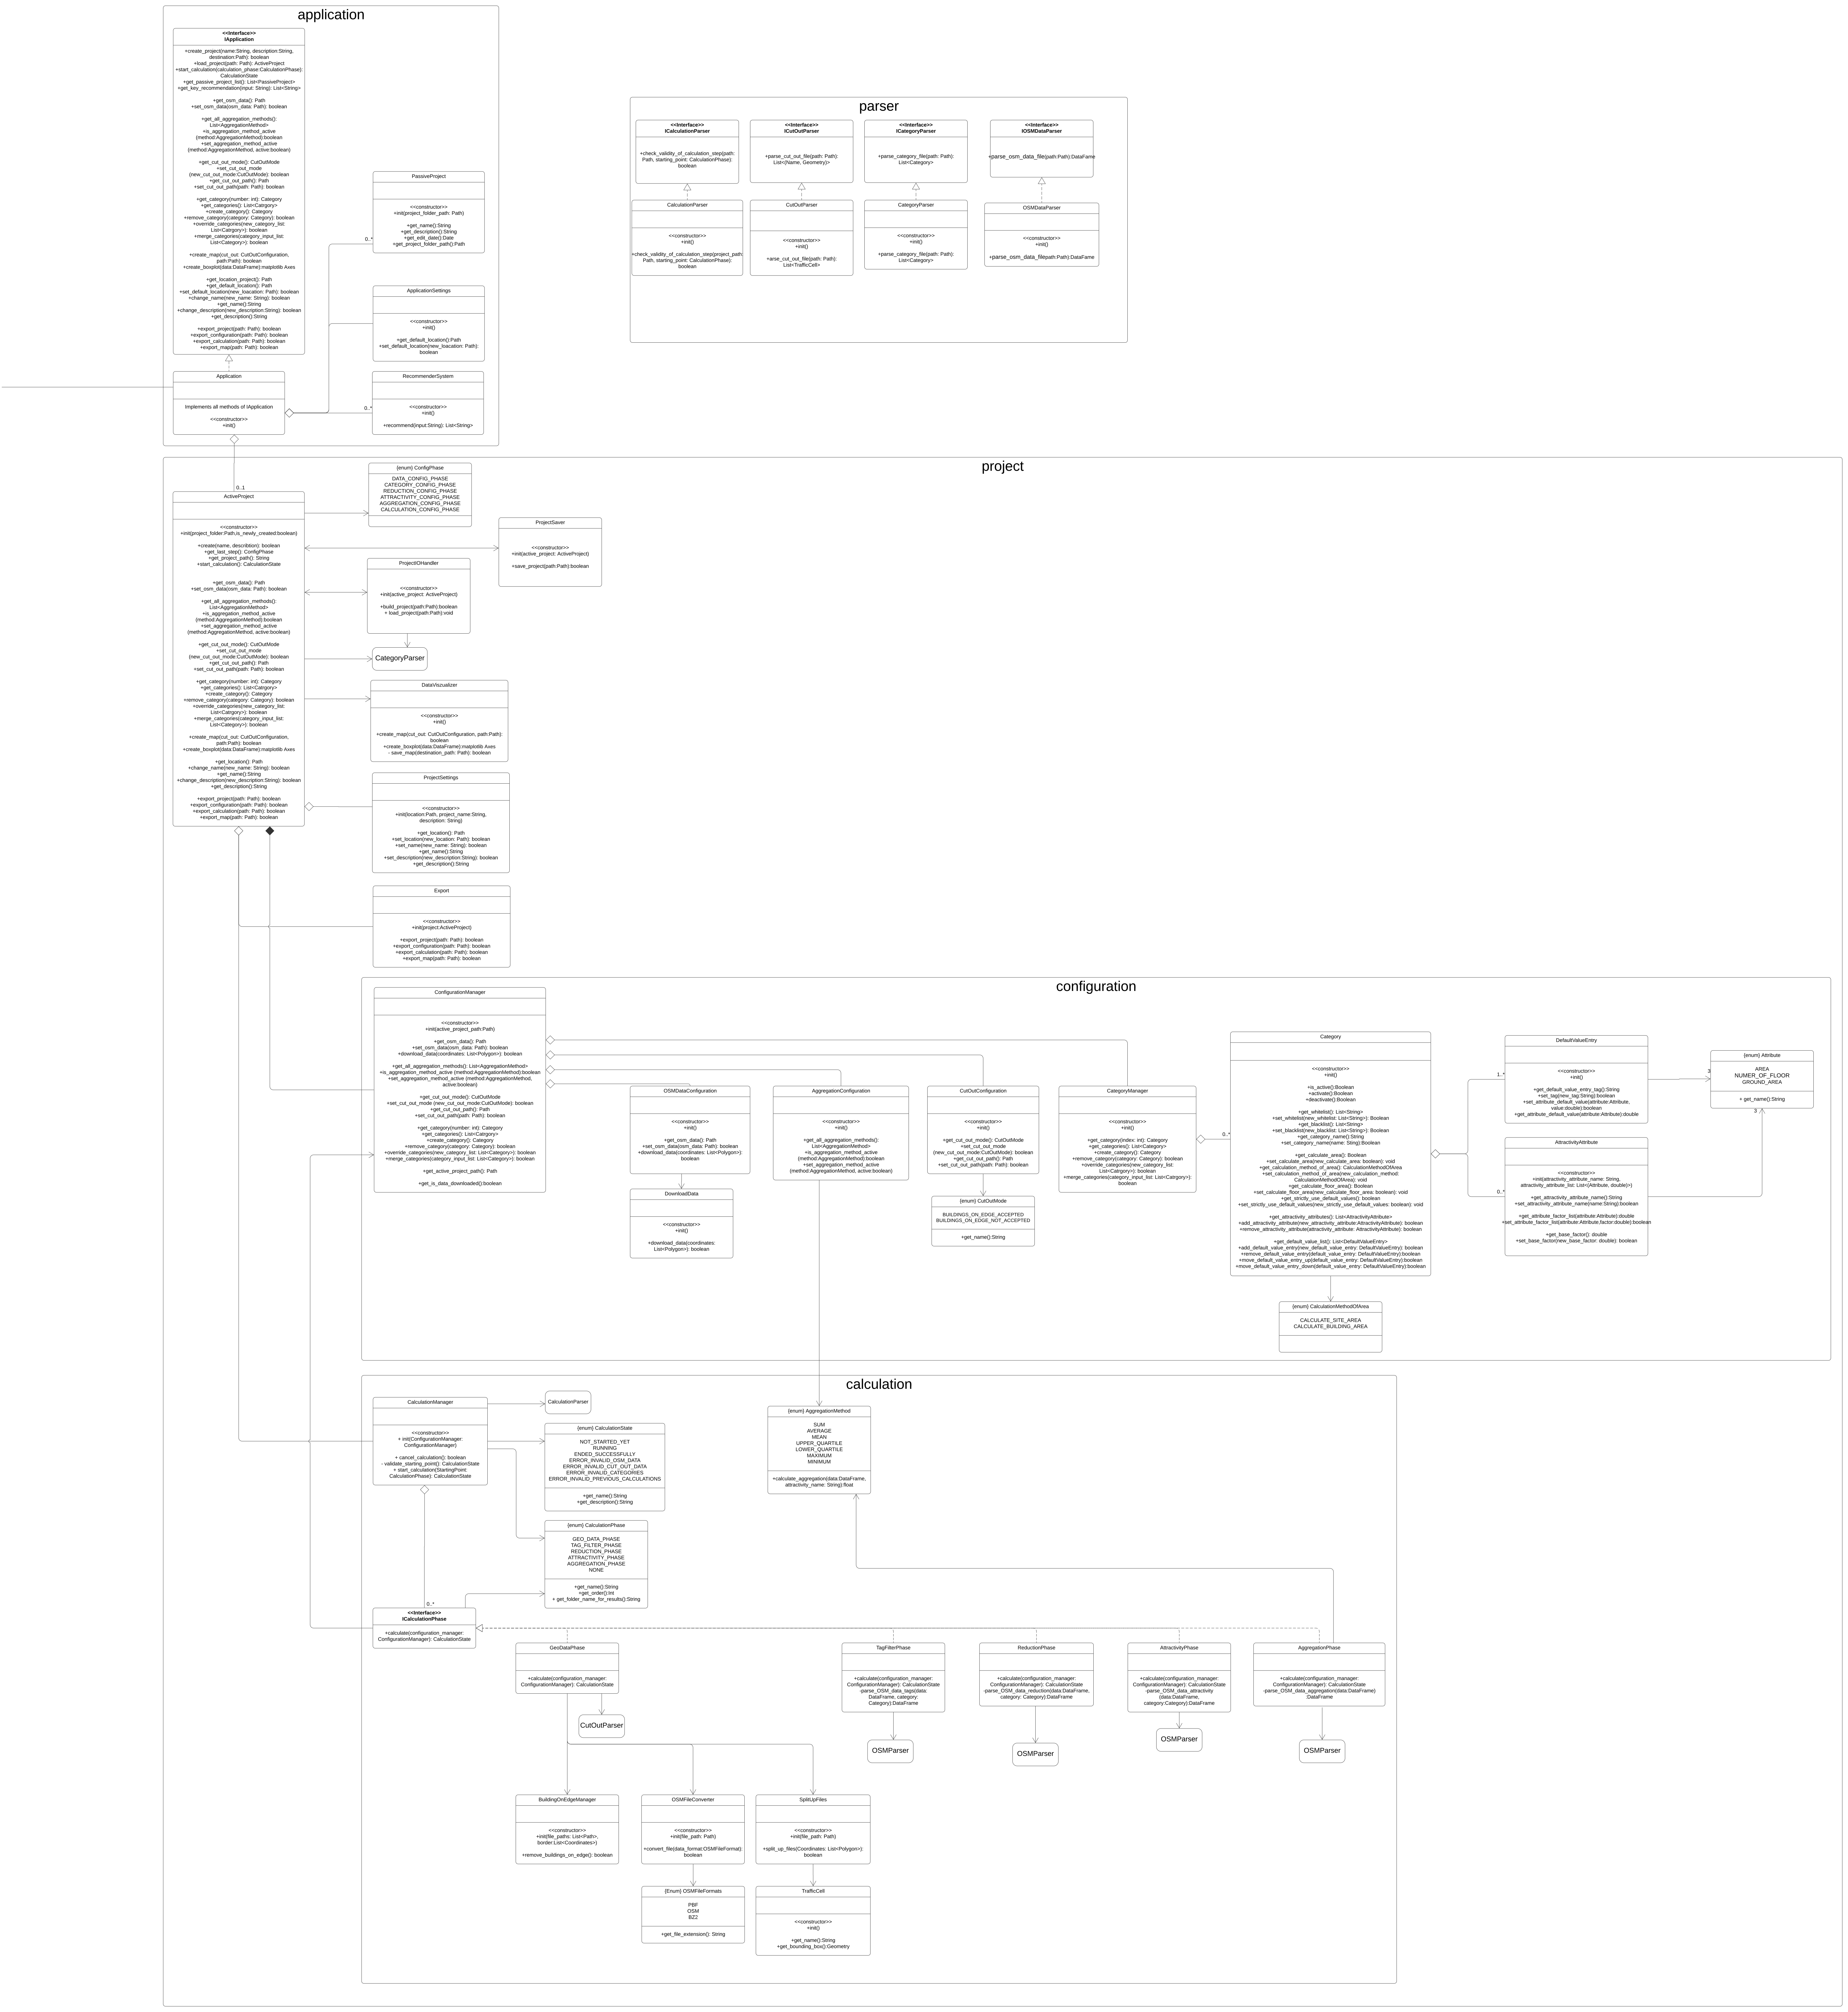
\includegraphics[width=0.8\textwidth]
        {pictures/model.png}
  \caption{Package: model}
  \label{fig:mvc}
\end{figure}
}

\hypertarget{popups}{
\begin{figure}[hbt!]
  \centering
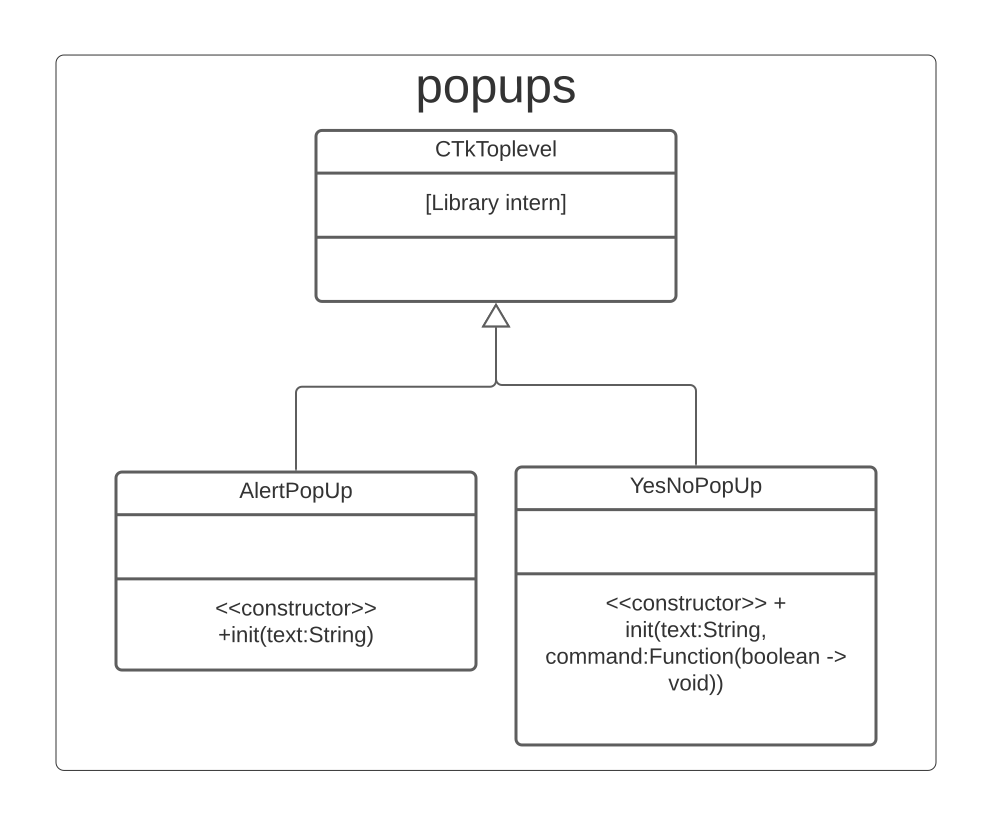
\includegraphics[width=0.5\textwidth]
        {pictures/popups.png}
  \caption{Package: popups}
  \label{fig:mvc}
\end{figure}
}

\hypertarget{states}{
\begin{figure}[hbt!]
  \centering
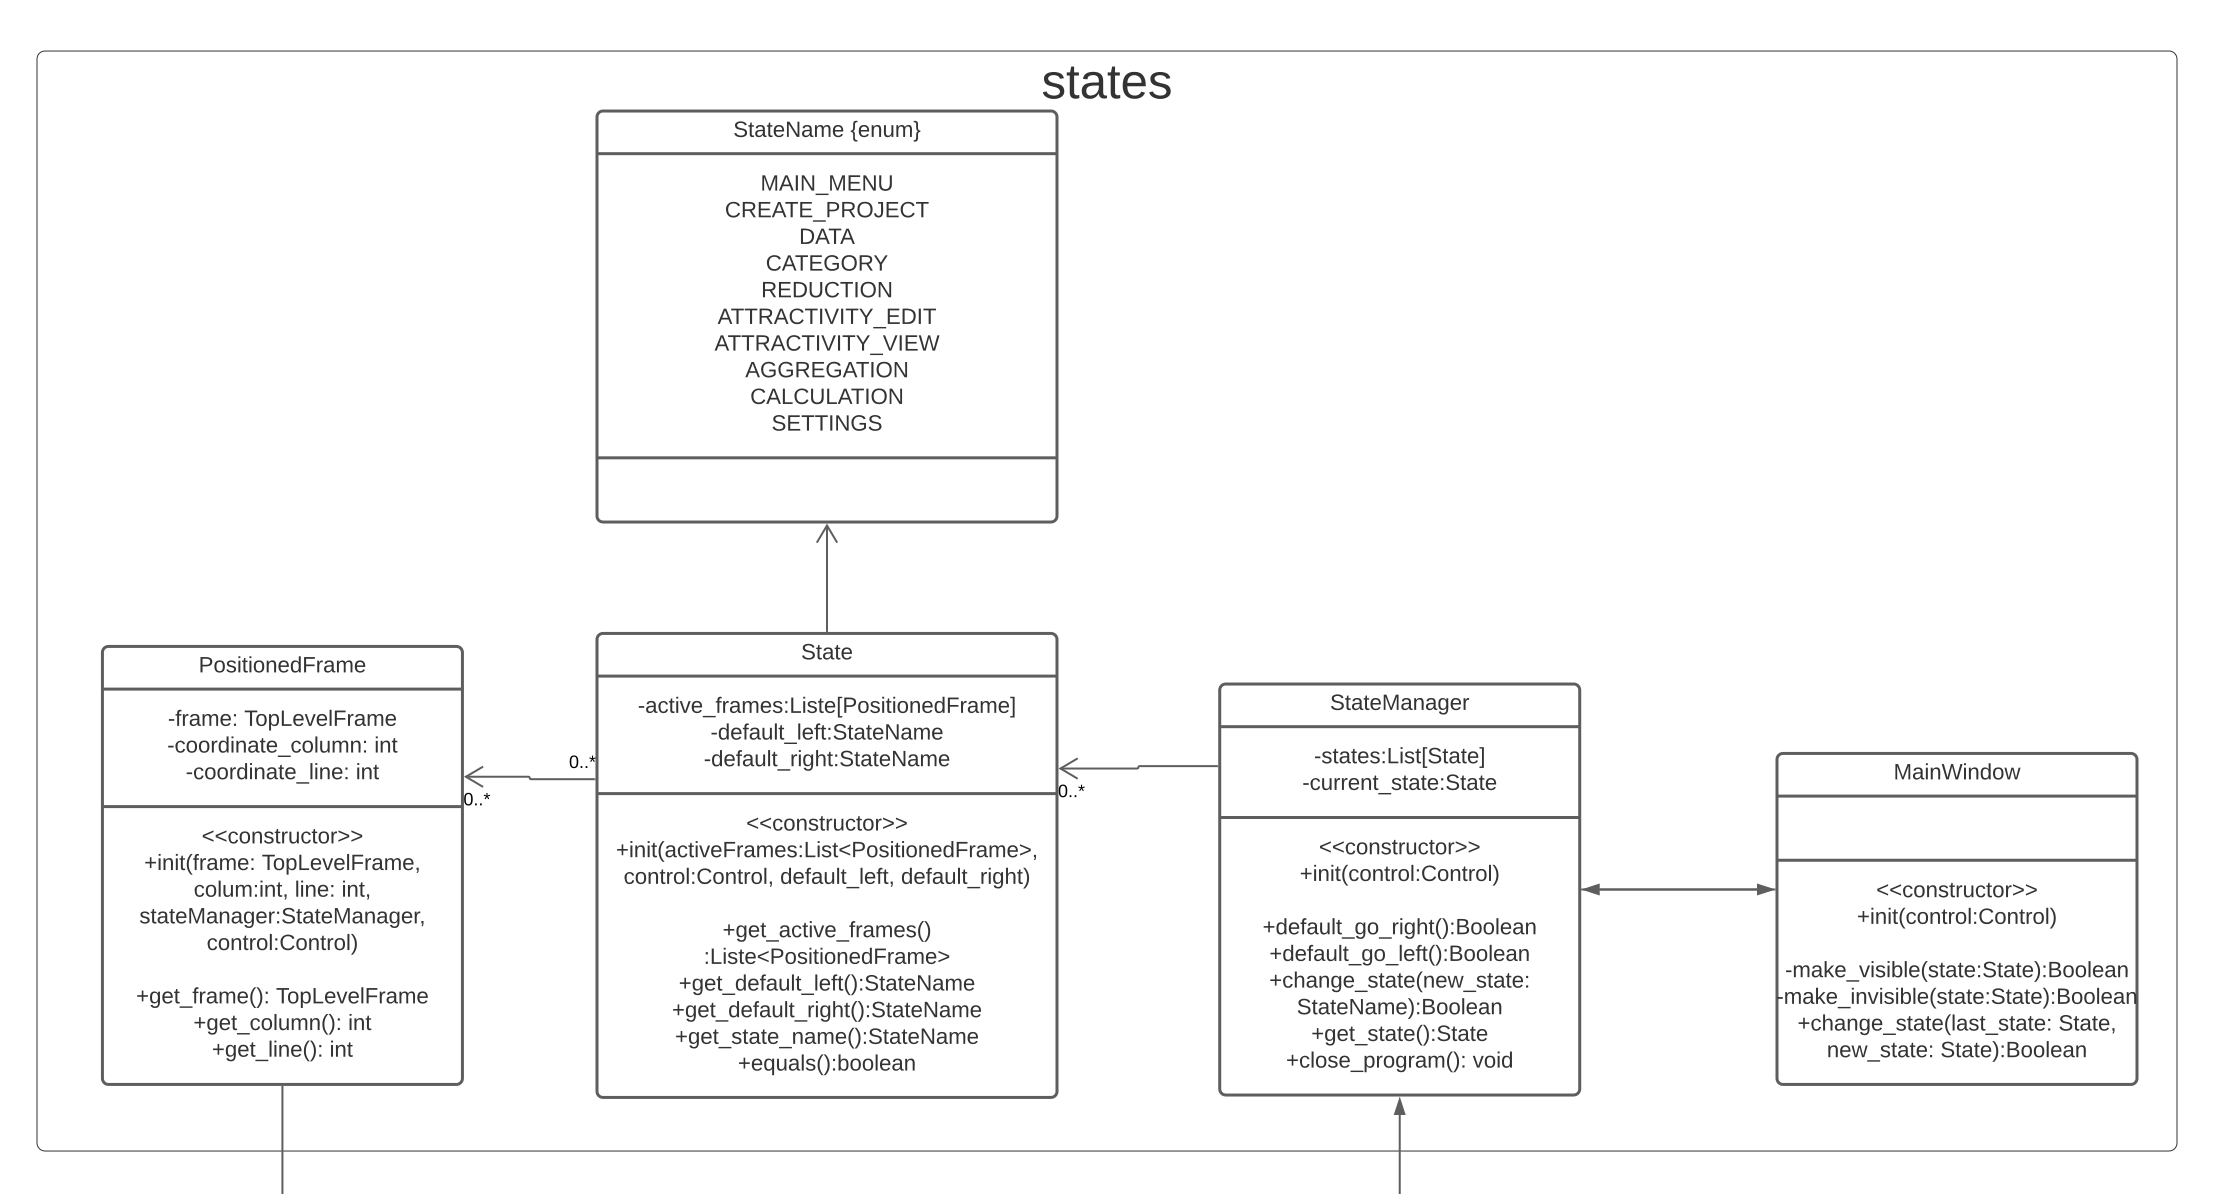
\includegraphics[width=0.8\textwidth]
        {pictures/states.png}
  \caption{Package: states}
  \label{fig:mvc}
\end{figure}
}

\hypertarget{toplevelframes}{
\begin{figure}[hbt!]
  \centering
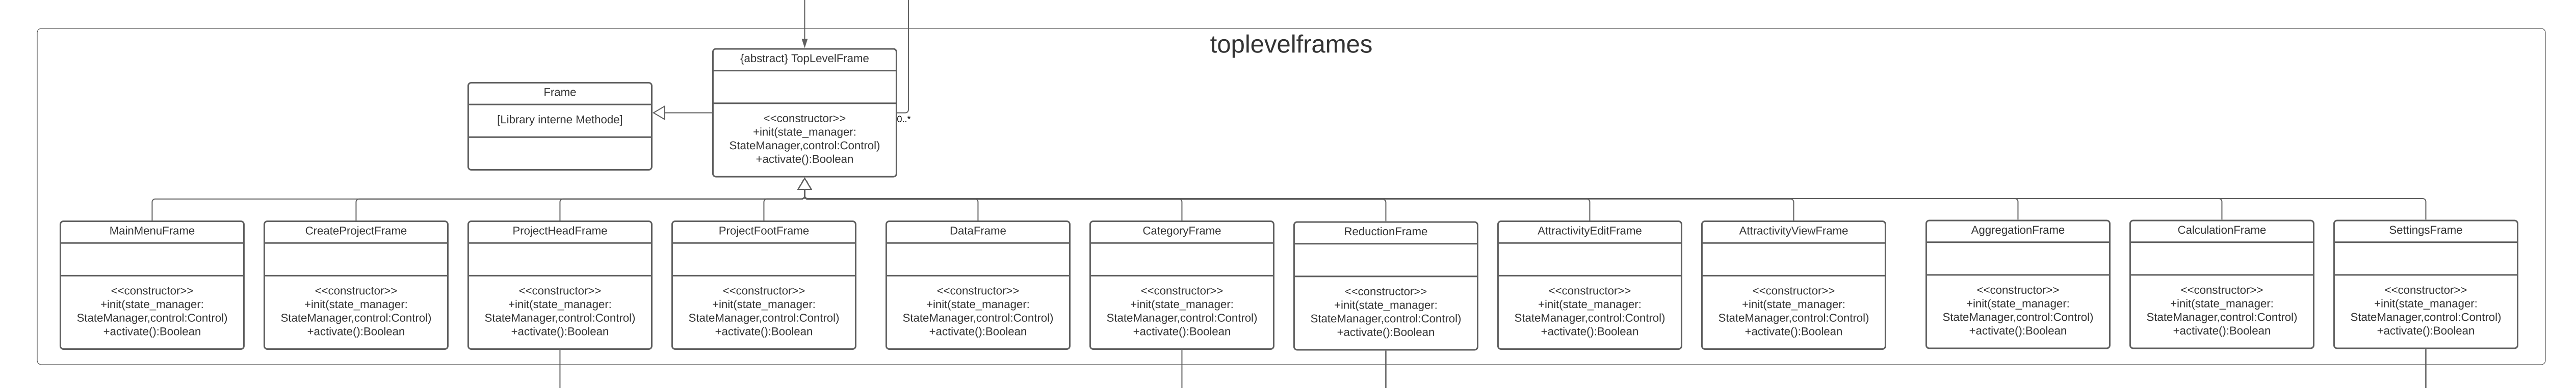
\includegraphics[width=0.8\textwidth]
        {pictures/toplevelframes.png}
  \caption{Package: toplevelframes}
  \label{fig:mvc}
\end{figure}
}

\hypertarget{utilityframes}{
\begin{figure}[hbt!]
  \centering
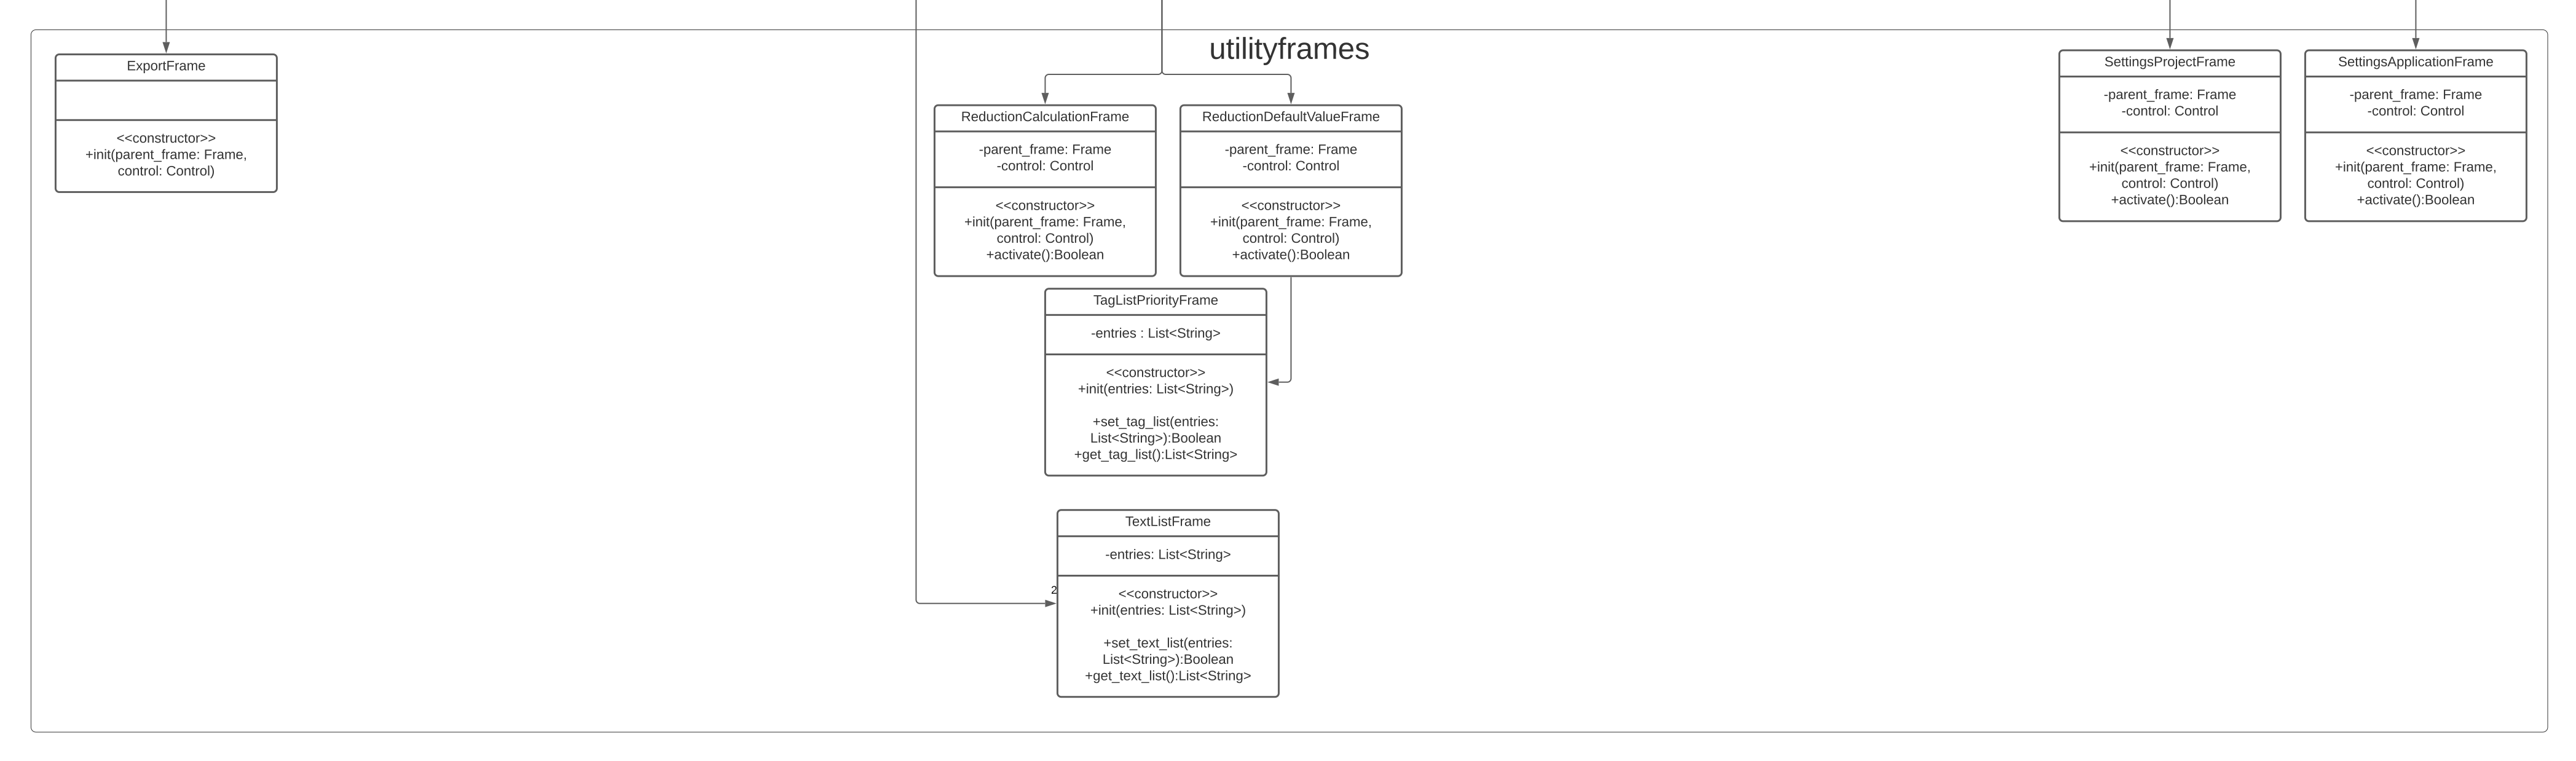
\includegraphics[width=0.8\textwidth]
        {pictures/utilityframes.png}
  \caption{Package: states}
  \label{fig:mvc}
\end{figure}
}

\hypertarget{application}{
\begin{figure}[hbt!]
  \centering
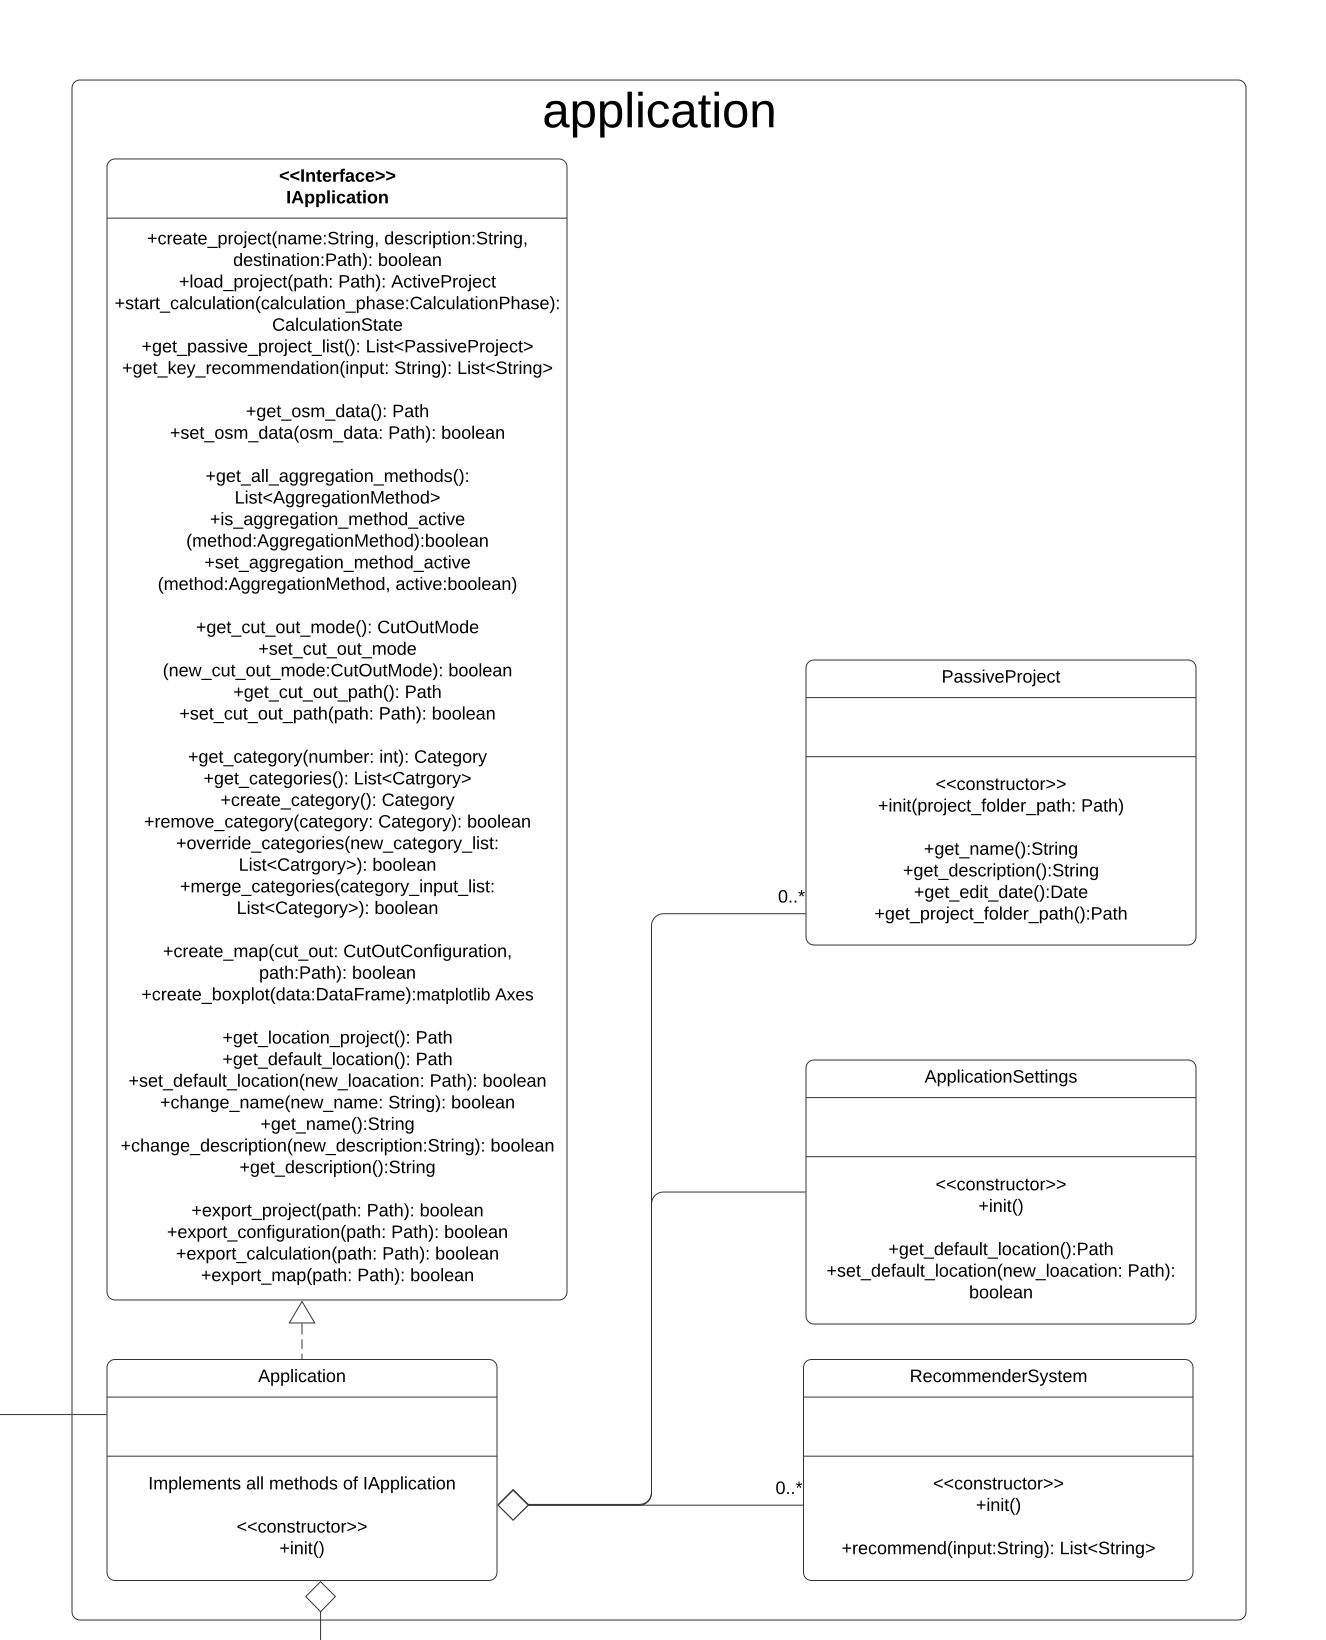
\includegraphics[width=0.8\textwidth]
        {pictures/application.png}
  \caption{Package: application}
  \label{fig:mvc}
\end{figure}
}

\hypertarget{parser}{
\begin{figure}[hbt!]
  \centering
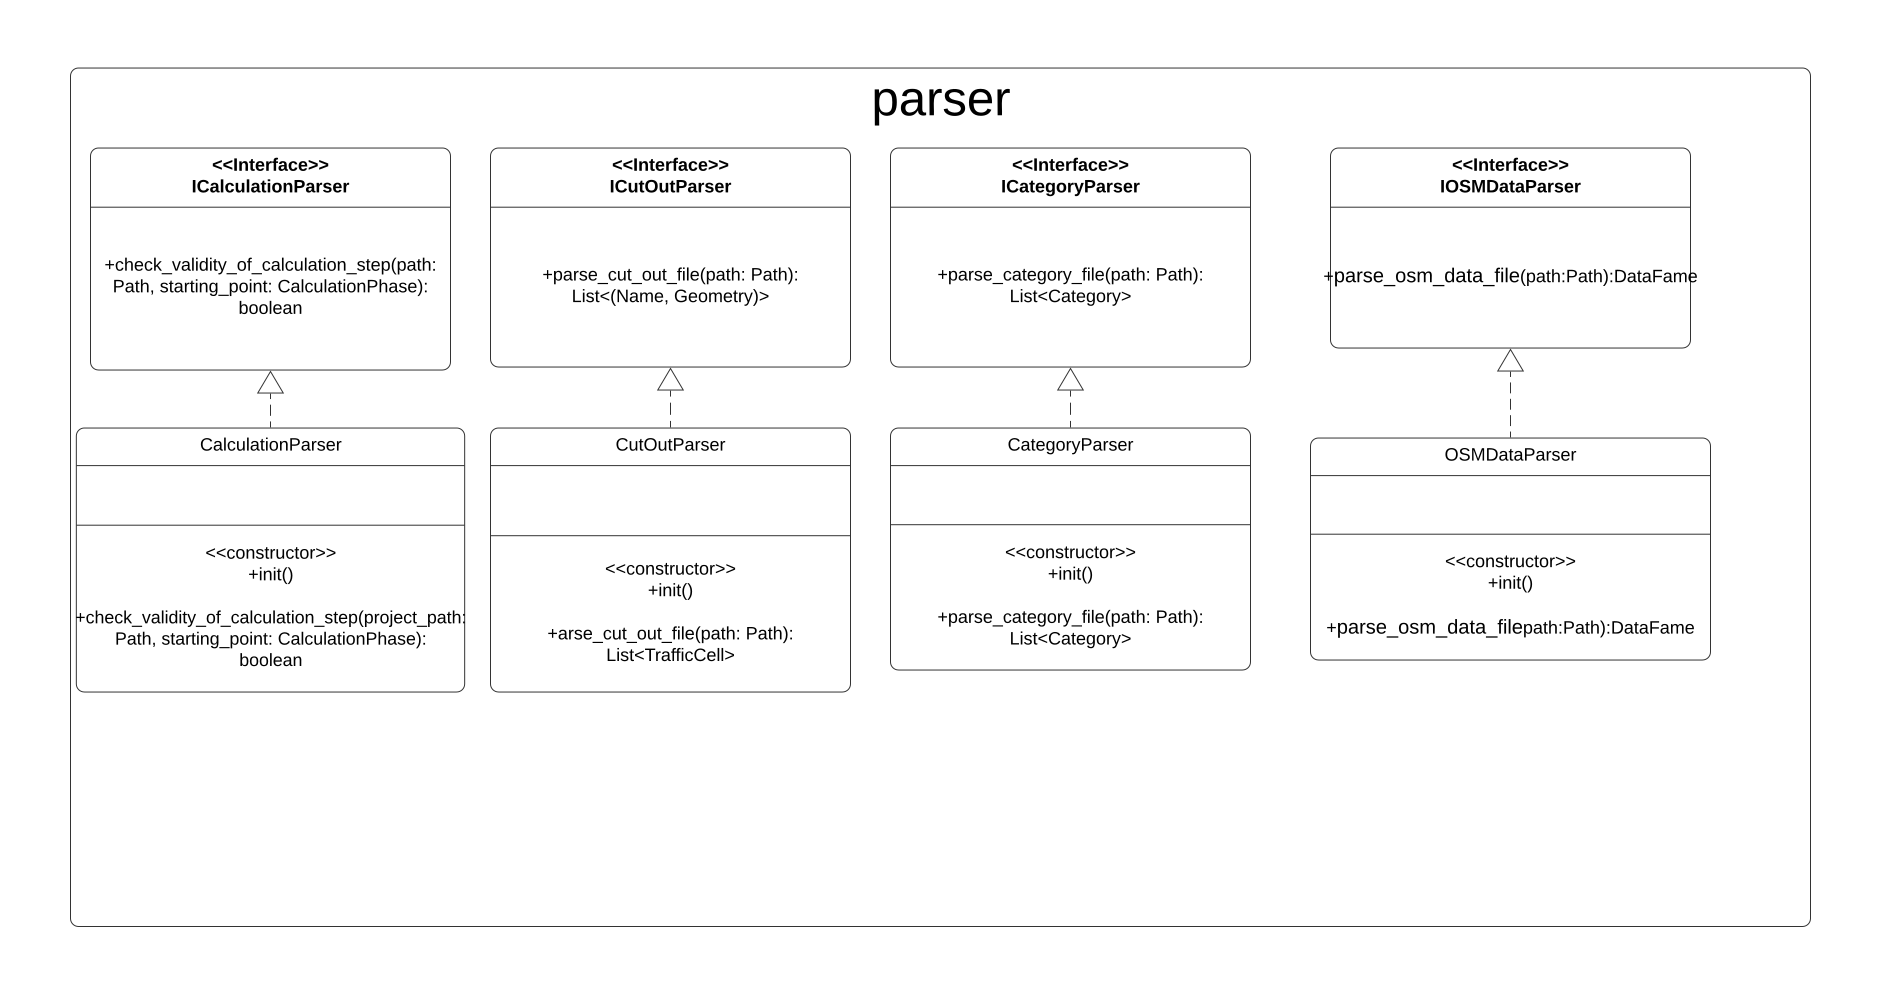
\includegraphics[width=0.7\textwidth]
        {pictures/parser.png}
  \caption{Package: parser}
  \label{fig:mvc}
\end{figure}
}

\hypertarget{project}{
\begin{figure}[hbt!]
  \centering
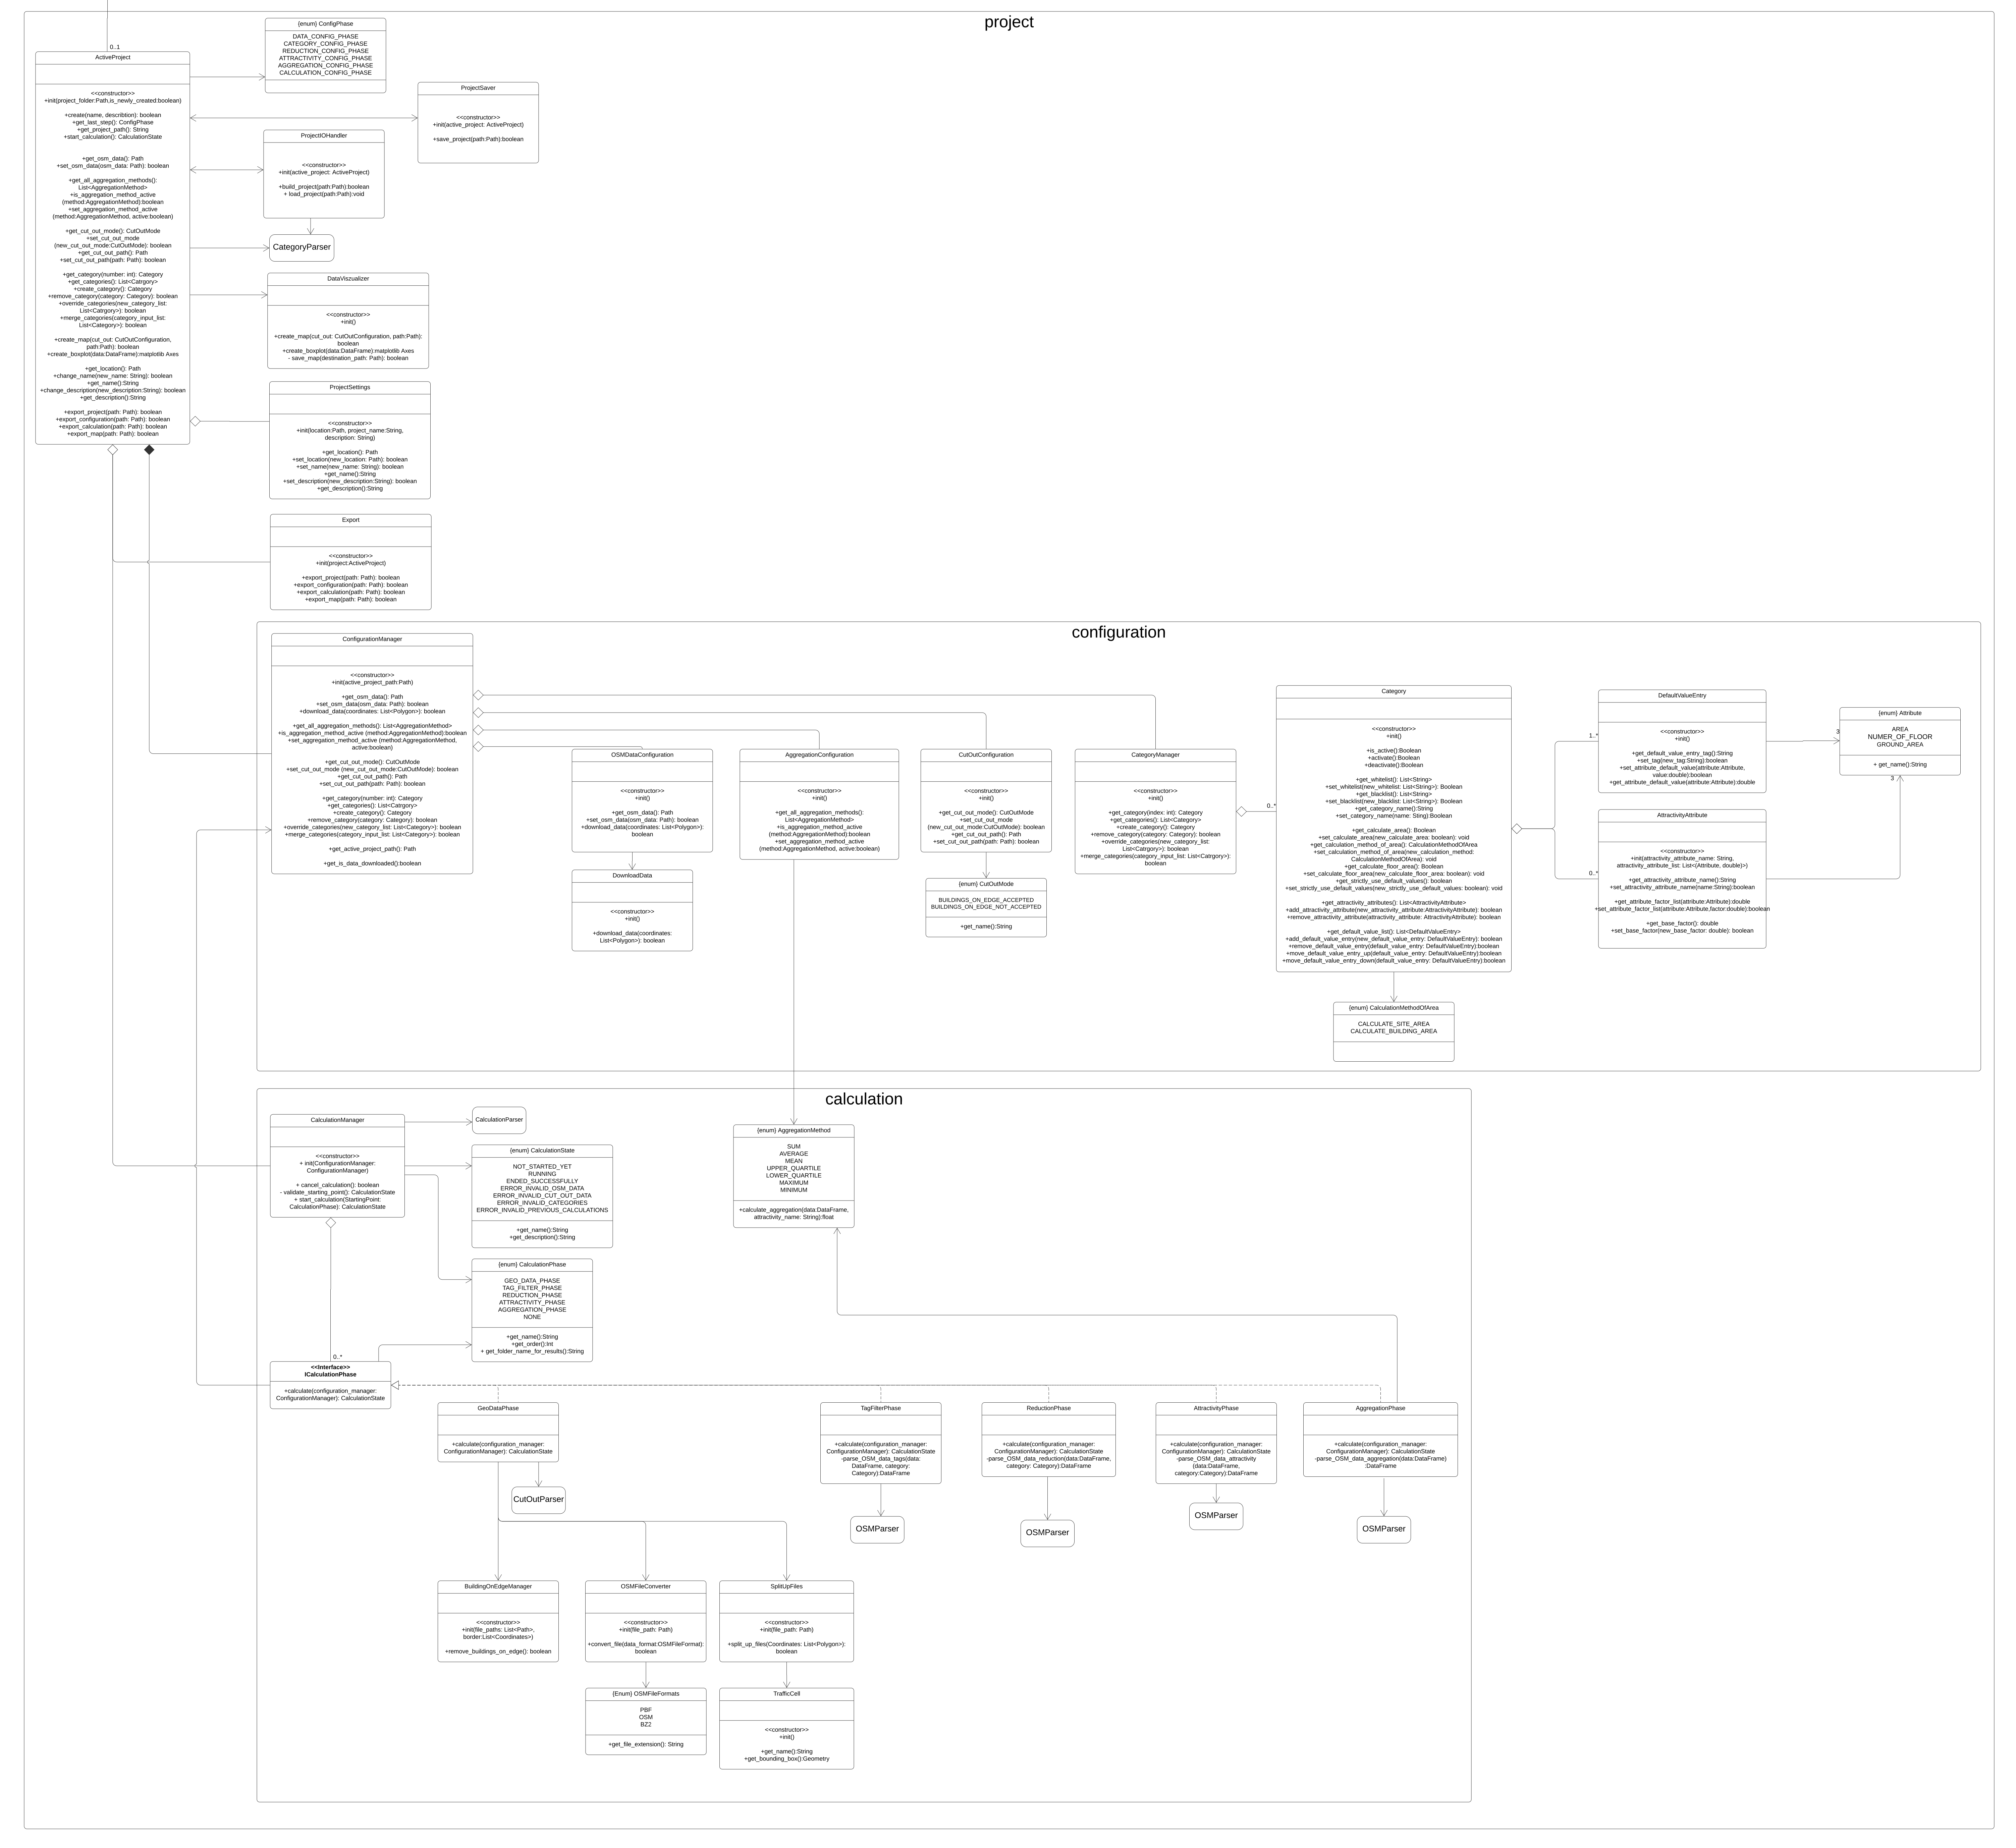
\includegraphics[width=0.8\textwidth]
        {pictures/project.png}
  \caption{Package: project}
  \label{fig:mvc}
\end{figure}
}

\hypertarget{configuration}{
\begin{figure}[hbt!]
  \centering
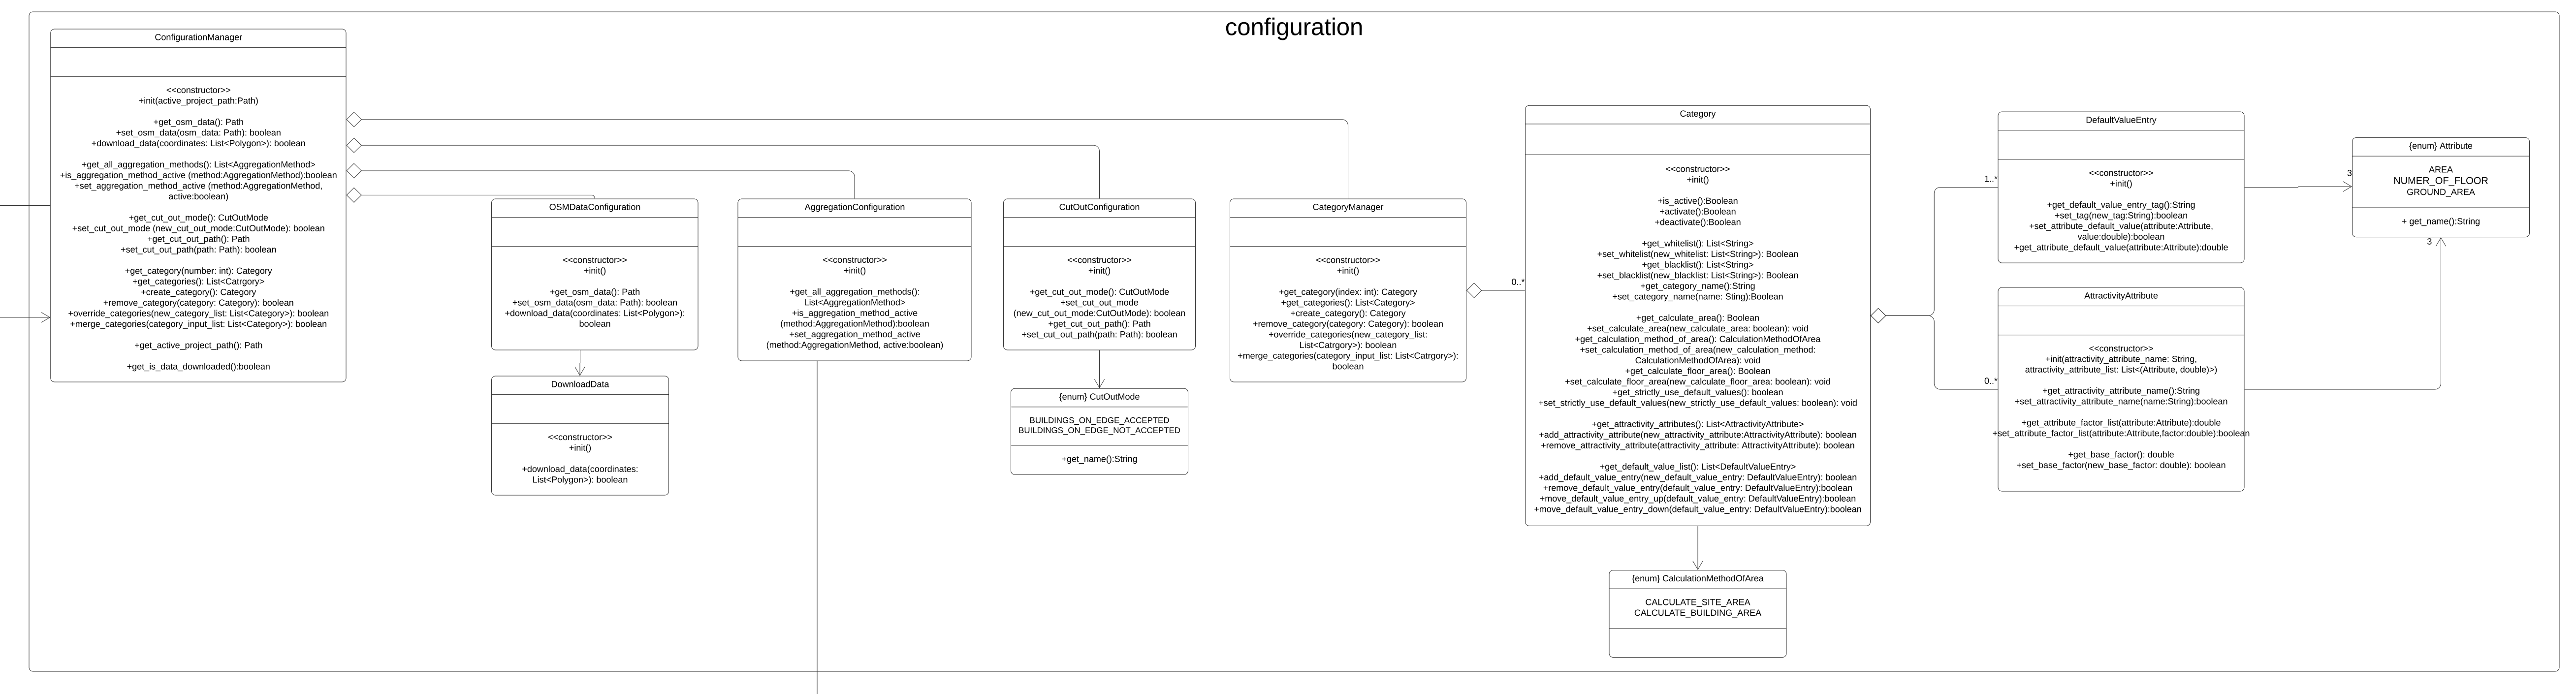
\includegraphics[width=0.8\textwidth]
        {pictures/configuration.png}
  \caption{Package: configuration}
  \label{fig:mvc}
\end{figure}
}

\hypertarget{calculation}{
\begin{figure}[hbt!]
  \centering
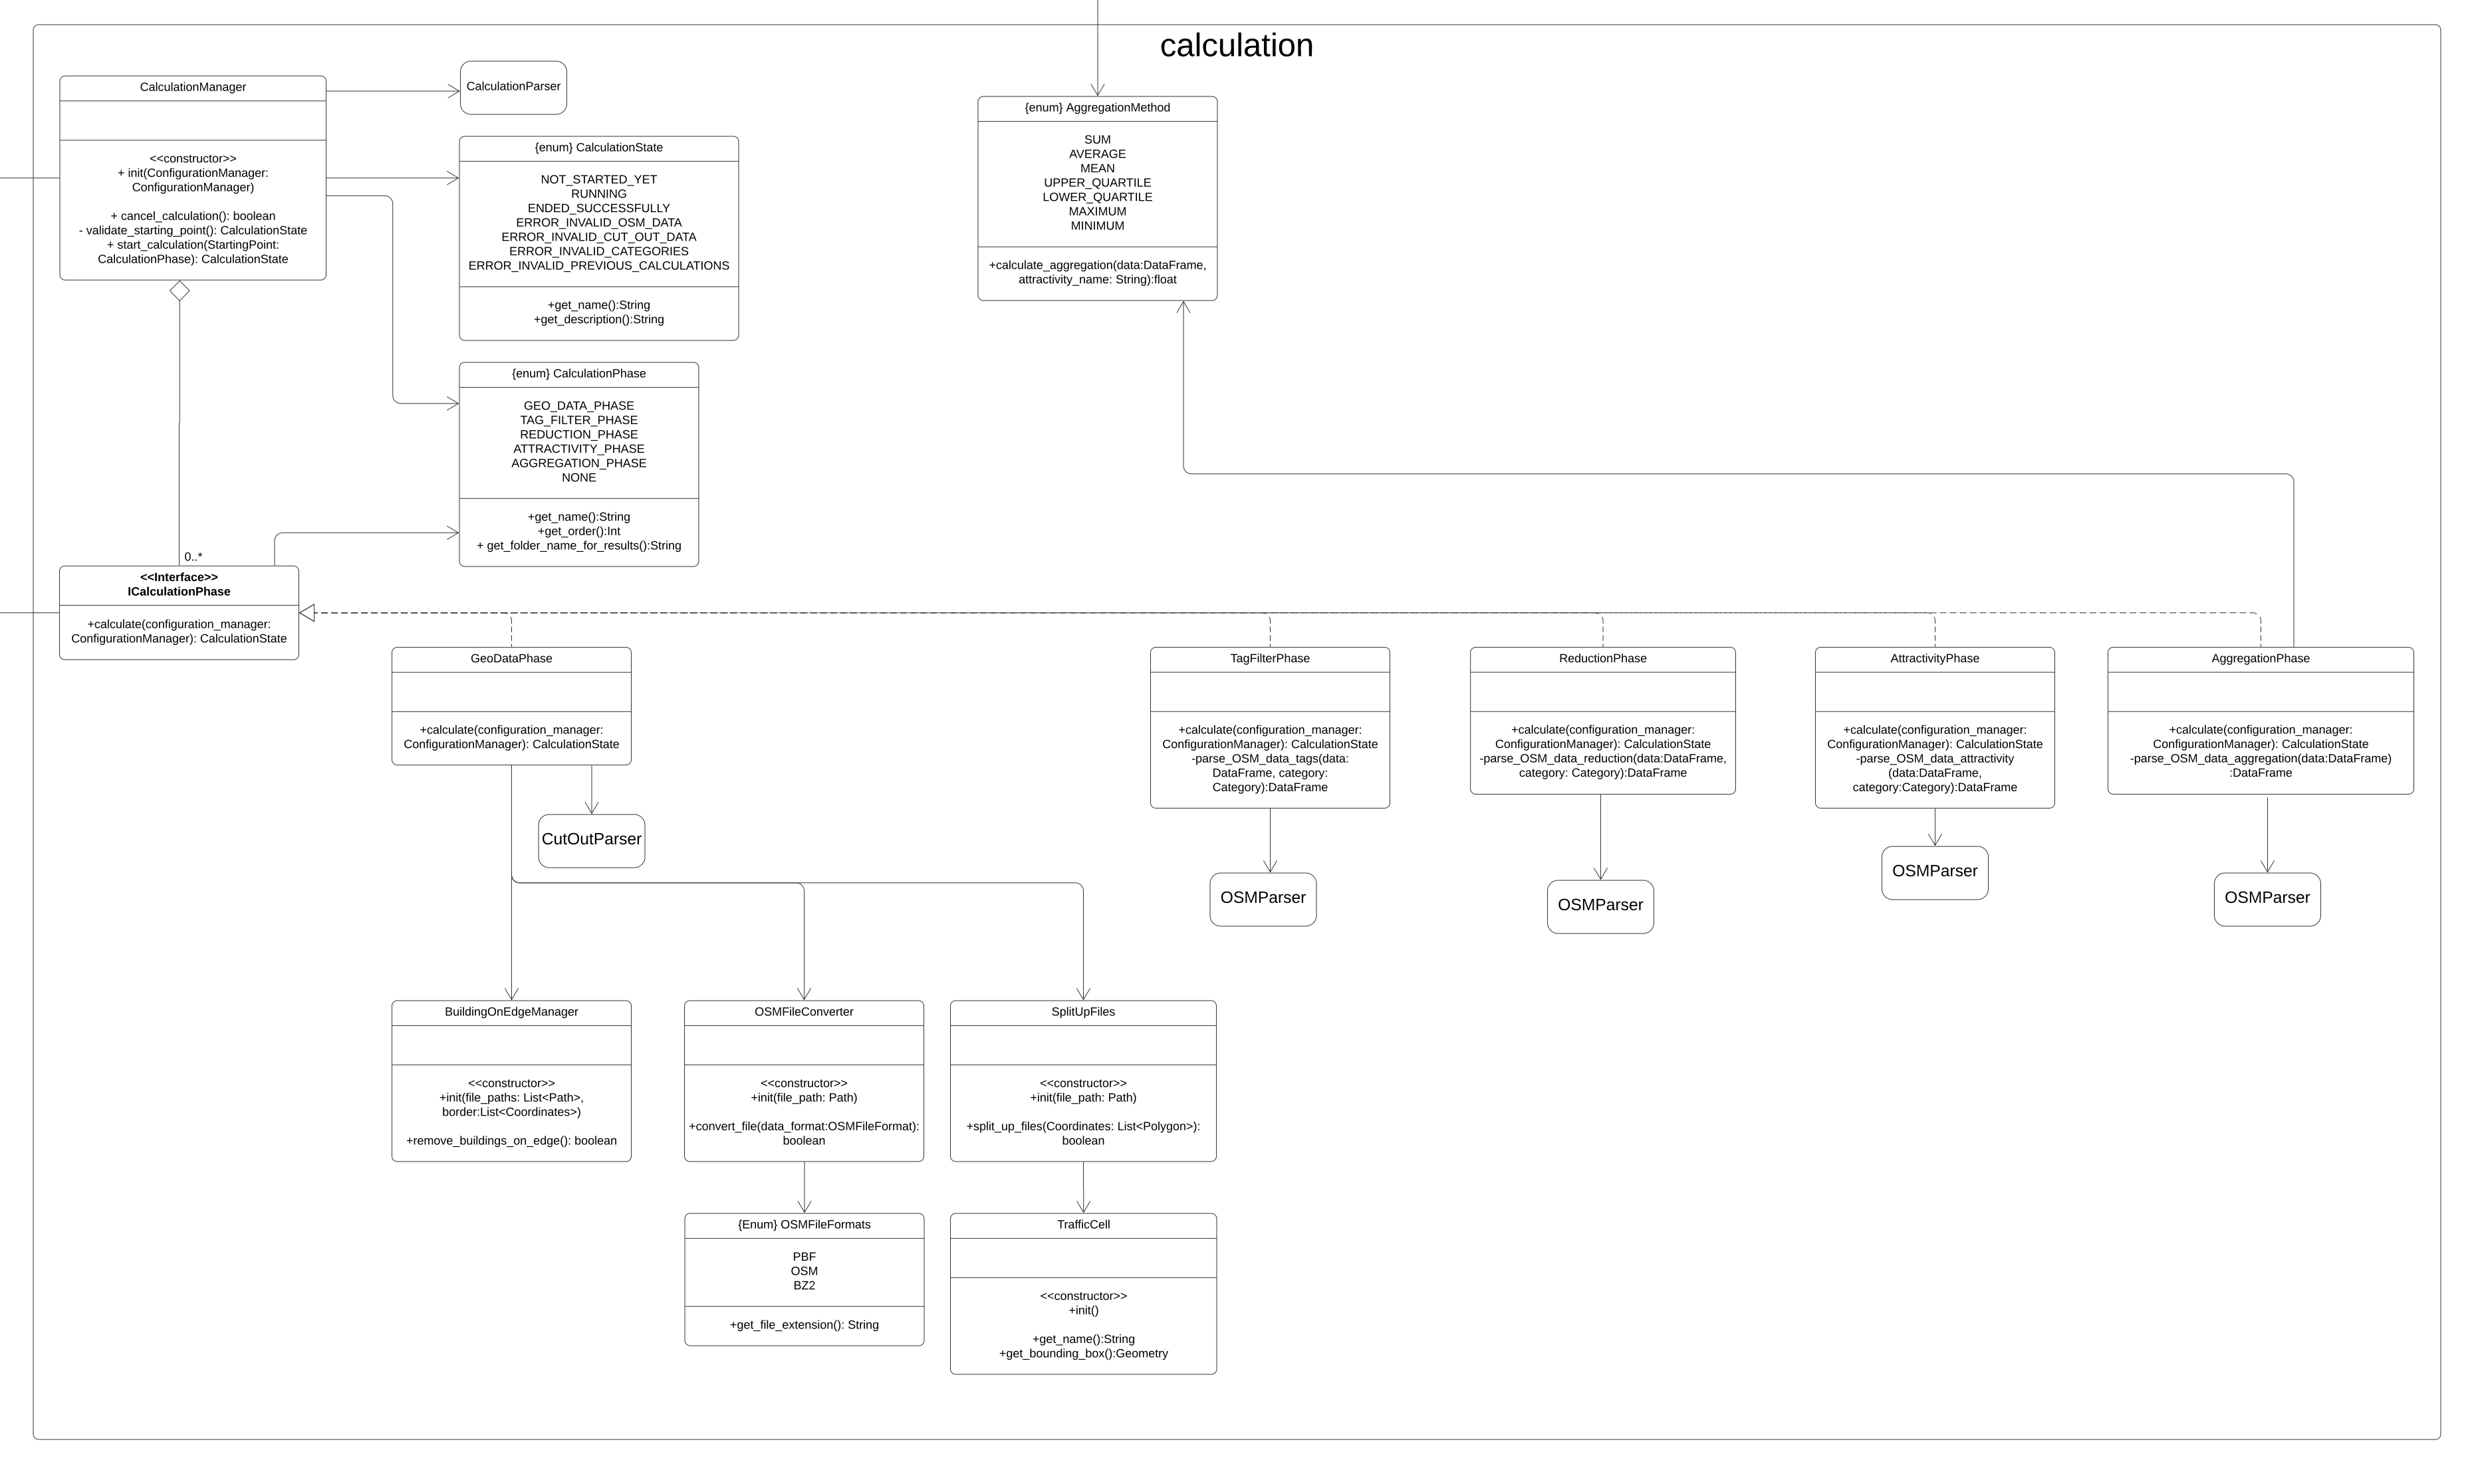
\includegraphics[width=0.8\textwidth]
        {pictures/calculation.png}
  \caption{Package: calculation}
  \label{fig:mvc}
\end{figure}
}



\chapter{Software Patterns}

\section{MVC}
This project uses the Model-View-Controller pattern as described in \ref{sec::mvc}.

\section{Facade}
\subsection{Definition}
The Facade-Pattern hides the complexities of the system providing an abstract class to the client that can access the system. This interface is implemented by using a single class providing the necessary functionality. This helps fighting code redundancy, makes creating new frames easier and therefore reduces debugging efforts.
\subsection{Usage}
This project uses the facade-pattern in the view-package. By implementing a parent providing basic-functionality to its children, code duplications implementing the same functionality can be avoided. Child classes can overwrite the given methods if necessary and implement new features and attributes.
A lot of view-classes implement only small tweaks in a default-functionality-environment while creating new windows. The AggregationFrame for example only has small functionality-tweaks to the SettingsFrame. The different appearance of the frames is implemented separately, but the base-functionality of e.g. pressing a button is implemented only once.


\chapter{Sequence Diagram}
The sequence diagram below (figure \ref{fig:sequencediagram}) shows how the application behaves when switching to the category frame and when the user creates a new category. This example shows two important mechanisms of our design:\\
Firstly, it shows how switching states works in the view. The StateManager is informed, when the state needs to be changed. It decides which frames must be shown to the user and forwards the request to the MainWindow. When a frame is activated, it's activate() method is invoked. \\
Secondly, the communication between the view, the control and the model is shown. Frames of the view message requests to the control. The control forwards the message to the model. The request is answered via return values.


\begin{sidewaysfigure}
\centering
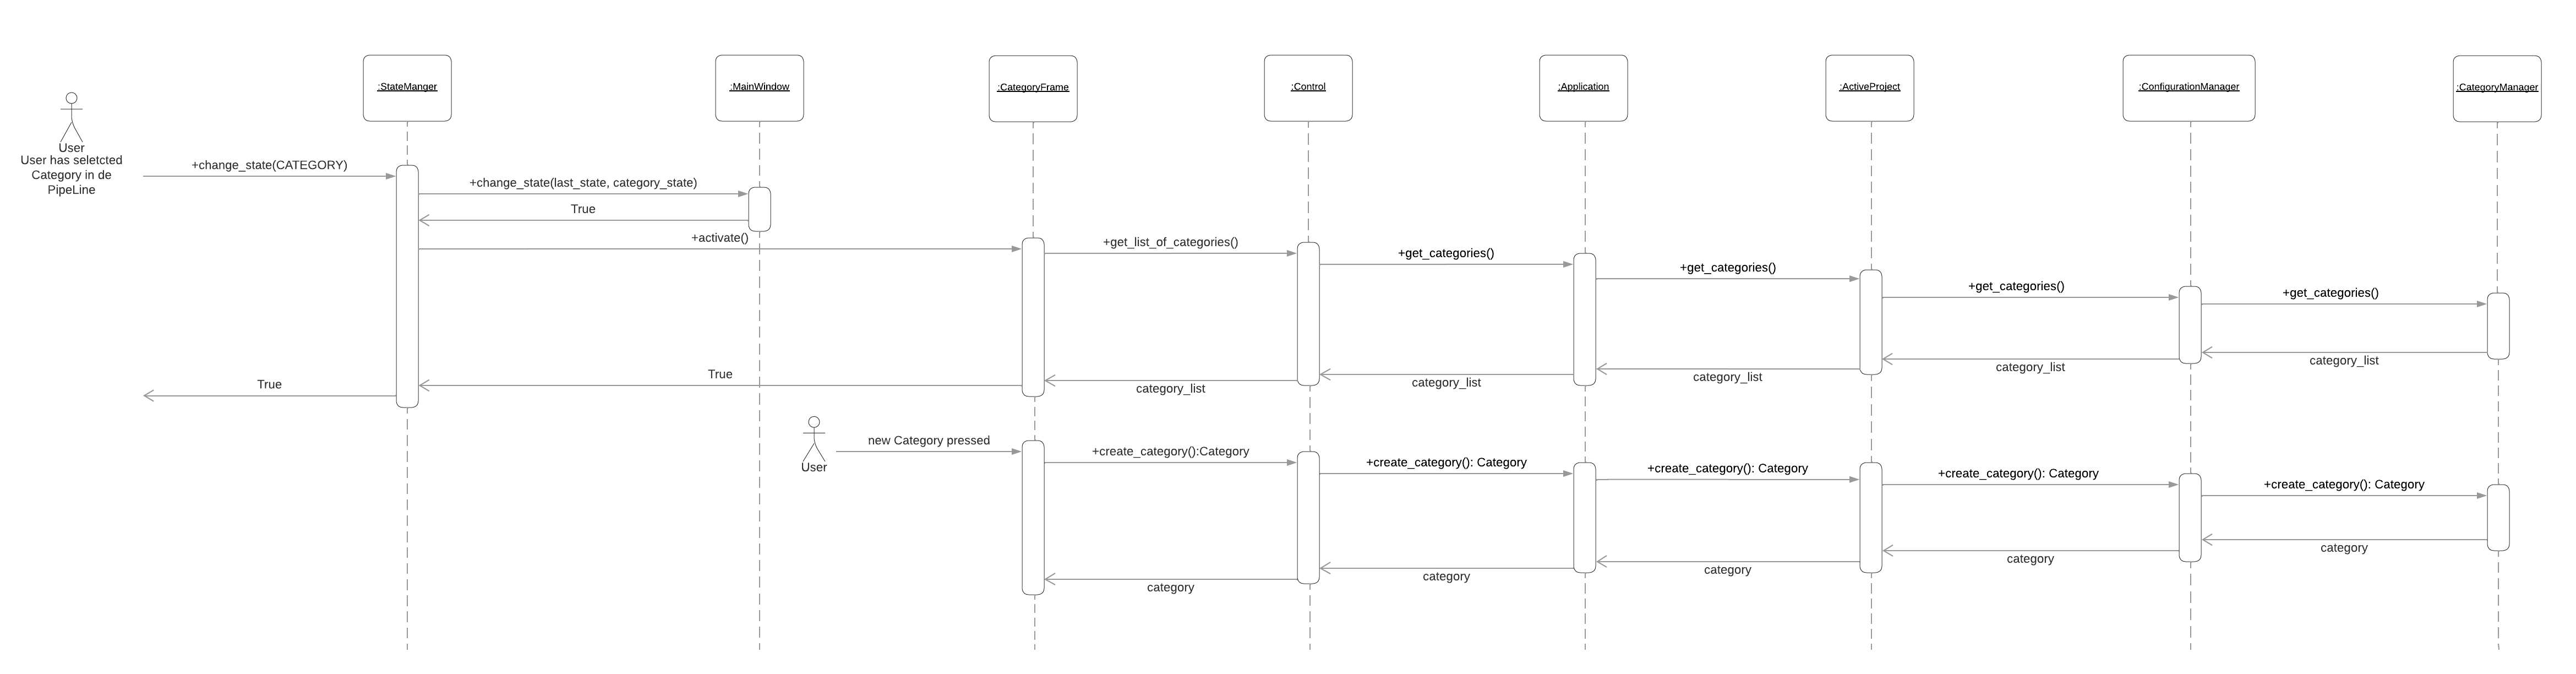
\includegraphics[width=1\textwidth]
        {pictures/sequenzdiagramm.png}
  \caption{sequence diagram}
  \label{fig:sequencediagram}
\end{sidewaysfigure}


\chapter{Libraries}

\section{Frontend and Dashboard}

\subsection{CustomTkinter}

\paragraph{What is CustomTkinter?}
\href{https://github.com/TomSchimansky/CustomTkinter}{CustomTkinter} is a python UI-library based on Tkinter, which provides new, modern and fully customizable widgets. They are created and used like normal Tkinter widgets and can also be used in combination with normal Tkinter elements. 

\paragraph{Why use CustomTkinter?}
We decided to use CustomTkinter as a UI-library, because TKinter is an easy to use library, which is standard in Python ecosystem.
But Tkinter alone looks a bit outdated, CustomTkinter provides Tkinter in a more modern look.

\paragraph{Why not use <insert Library name here>?}
CustomTkinter had a couple of alternatives that could have been used but all of them had disadvantages that made them worse in our use case than CustomTkinter. 
  
\textbf{Tkinter}
\begin{itemize}
    \item Same features as CustomTkinter but has a more aged look.
\end{itemize}
  
\textbf{Pyqt5}
\begin{itemize}
    \item Offers more features compared to CustomTkinter, but is more complicated and these additional features are not needed in our project.
    \item PyQT5 is not free for commercial use, it's better to have a more lenient licence.
\end{itemize}
\textbf{Kivy}
\begin{itemize}
    \item Offers more features compared to CustomTkinter, but is more complicated and these additional features are not needed in our project. 
\end{itemize}


\subsection{Seaborn}
\paragraph{What is Seaborn?}
\href{https://seaborn.pydata.org/}{Seaborn} is a Python data visualization library based on matplotlib. It provides a high-level interface for drawing attractive and informative statistical graphics.

\paragraph{Why use Seaborn?}
In our application we use Seaborn to visualize the endresult of the calculation.

\paragraph{Why not use <insert Library name here>?}
The only really other alternative to Seaborn is matplotlib which can do the same as Seaborn, but Seaborn is more easily usable then matplotlib, furthermore Seaborn uses matplotlib in the background to create and visualize their results.




\section{Backend}
% Ist es besser hier nach Model, View und Controller zu sortieren?

\subsection{osmium-tool}

\paragraph{What is osmium-tool?}
\href{https://osmcode.org/osmium-tool/}{Osmium}
is a versatile command line tool for working with OpenStreetMap data. It includes many useful functions for manipulating OSM data and often outperforms similar tools.

\paragraph{Why use osmium-tool?}
In our application we will deal with very large OSM-Data files.
The osmium-tool allows us to convert from one OSM-Data file format to another one. 
Furthermore it can be used to split large OSM-Data files into multiple smaller ones, which we will use to split the OSM-Data into the previously defined 
\hyperref[sec:Glossary]{traffic cells}.

\paragraph{Why not use <insert Library name here>?}
Osmium-tool doesn't really have competitors in it's space, there aren't any mature python libraries which can cut OSM-data files like osmium-tool.
Though there are libraries/application written in different languages that can do what Osmium-tool does, such as Osmosis or osmfilter.
But they are slower or require additional software such as java.


\subsection{Osmium}

\paragraph{What is Osmium?}
The \href{https://osmcode.org/libosmium/}{Osmium} Library has extensive support for all types of OSM entities: nodes, ways, relations, and changesets. It allows reading from and writing to OSM files in XML, PBF, and several other formats, including change files and full history files. Osmium can store OSM data in memory and on disk in various formats and using various indexes.

\paragraph{Why use Osmium?}
In out application we use Osmium to parse buildings out of the OSM-Data file.

\paragraph{Why not use <insert Library name here>?}
Osmium had a couple of alternatives that could have been used but all of them had disadvantages that made them worse in our use case than Osmium. 
  
\textbf{OSMnx}
\begin{itemize}
    \item Is more used for network, such as street networks. 
    \item When trying it out, it was hard to work with.
\end{itemize}


\textbf{Pyrosm}
\begin{itemize}
    \item Pyrosm isn't as active developed as it used to be, no support for newer python version, dependencies use old version.
    \item Pyrosm wasn't compatible with the rest of libaries we use, since it depends on old version of libaries.
\end{itemize}

\subsection{Psutil}
\paragraph{What is Psutil?}
Psutil (process and system utilities) is a cross-platform library for retrieving information on running processes and system utilization (CPU, memory, disks, network, sensors) in Python. It is useful mainly for system monitoring, profiling and limiting process resources and management of running processes. 

\paragraph{Why use Psutil?}
In our Project we use Psutil to monitor the RAM usage, this is required for decision like: how much OSM-Data do we load simultaneous in the RAM?

\paragraph{Why not use <insert Library name here>?}
Psutil is a small  library, that does what it promises to do, it is not needed to find a "better" library.

\subsection{Sphinx}

\paragraph{What is Sphinx?}
Sphinx is a documentation generator written and used by the Python community, it makes it easy to create intelligent and beautiful documentation.
It can generate web pages, printable PDFs, documents for e-readers (ePub), and more all from the same sources

\paragraph{Why use Sphinx?}
Sphinx allows us to easily document our code and make this beautiful document.

\paragraph{Why not use <insert Library name here>?}
Sphinx is industry standard when it comes to generating documenting from your code.

\subsection{osmnx}

\paragraph{What is osmnx?}
OSMnx is a Python package that lets you download geospatial data from OpenStreetMap and model, project, visualize, and analyze real-world street networks and any other geospatial geometries. You can download and model walkable, drivable, or bikeable urban networks with a single line of Python code then easily analyze and visualize them. You can just as easily download and work with other infrastructure types, amenities/points of interest, building footprints, elevation data, street bearings/orientations, and speed/travel time.

\paragraph{Why use osmnx?}
In our project we use use osmnx to download OSM Data to the project(Desirable criterion).

\section{Miscellaneous}
The Previously described libraries have many dependencies, that may also be used such as:
\begin{itemize}
    \item tkinter
    \item geopandas
    \item numpy
    \item shapely
    \item folium
    \item sphinx-enum-extend
    \item sphinx-book-theme 
    \item etc.
\end{itemize}



\chapter{Class Descriptions} \label{sec::descriptions}
\section{Notation}
Details of the used notation

\section{Controller-Classes}

\section{Model-Classes}

\section{View-Classes}



\chapter{Glossary}

\section*{Aggregation}
Process summarizing multiple attractivity-attributes from a single traffic-zone

\section*{Aggregation-Process}
Maps a set of attractivity-attributes onto a number, e.g. by adding or multiplying.

\section*{Attractivity-Attribute}
Attribute of a geographical object. Describes the attractivity of a place in terms of a certain action. Is calculated by using attributes.

\section*{Attribute}
Attribute of an OSM-Element. Is calculated during the point-reduction-phase by using OSM-Tags.

\section*{Calculation-Phase}
Continuous phase of the calculation-process. Different phases: OSM-Data, local filtering, tag filtering, point-reduction, attractivity-calculation and aggregation.

\section*{Checkbox}
Box representing a binary. By ticking the box, the according option is chosen.

\section*{Dropdown}
Describes a graphical element to navigate a GUI. An element or function can be chosen from the given list.

\section*{Explorer}
OS-tool to navigate and choose data from the disc.

\section*{Geofilter}
Process matching OSM-objects to geographical zones.

\section*{GUI}
GUI is the abbreviation for "Graphical User Interface".

\section*{Instance}
Differentiates between smaller and larger instances. Small instances describe data reaching 250 MB at max. Larger instances exceed this value.

\section*{Category}
Organises OSM-elements. A category defines a set of OSM-elements with their according characteristics.

\section*{Button}
Component of the GUI providing reactions and general interaction with the user.

\section*{Configuration-Phase}
Part of the Configuration of a project.

\section*{OSM}
Abbreviation for "Open Street Map". OSM is an open-source project collecting and publishing geodata for free.

\section*{OSM-file}
File containing OSM-objects.

\section*{OSM-object}
Entry of the OSM-database. Defined by its tags.

\section*{Project}
Organisational unit. Contains all related configurations.

\section*{Project-Folder}
Directory. Organises the configuration-files of a project.

\section*{Default folder}
Directory that stores projects file by default.

\section*{Point-Reduction}
Process mapping buildings to points. Each point has a certain set of attributes.

\section*{Local Filter}
Method describing a geofilter. Decides if OSM-elements at the edge of zones belong to the chosen area. 

\section*{Repository}
Server storing and managing objects, datasets, files and code.

\section*{Page}
Part of the GUI, that is shown at once.

\section*{Default-Category}
Each project has these categories by default.

\section*{Tag}
Characteristic of an OSM-object. Contains a 'key' and 'value'.

\section*{Tag-Filter}
Process separating OSM-Elements into certain group by checking their tags.

\section*{Investigated Area}
Zone investigated by the application. Joined set of disjunct traffic-cells. Is defined by using a local-filter.

\section*{Traffic Cell}
Refers to a spatially defined part of an investigated area that serves as a reference unit in traffic analysis and traffic forecasting.

\section*{Windows}
Windows is an operating system for computers and laptops.


\end{document}
